%  http://latex-beamer.sourceforge.net/

%\documentclass[landscape]{foils}

%\documentclass{beamer}
%\documentclass[handout]{beamer}     % TO PRINT PRESENTATION HANDOUT
\documentclass[xcolor=dvipsnames]{beamer}  % ALLOWS CHANGE IN COLOR

\usepackage{color}

\usepackage{pifont} %para tener la ballot cross \ding{55}

\usepackage{beamerthemesplit}
\usepackage{url}
\usepackage{ae} % or {zefonts}
\usepackage[T1]{fontenc}
\usepackage[ansinew]{inputenc}
\usepackage[spanish]{babel}

\usepackage{graphicx}
%\graphicspath{"c:/data"}
\usepackage{color}
%\usepackage[colorlinks]{hyperref}
\usepackage{tikz} % Easier syntax to draw pgf files (invokes pgf automatically)
\usetikzlibrary{arrows,shapes.geometric}
%\usepackage{pgfmath}


%\usecolortheme{crane}     %Color yellow
%\usetheme{Warsaw}
\usecolortheme[named=Gray]{structure}

\useoutertheme[footline=empty]{}  % PUTS COLORED LINE AT FOOT WITH TITLE, AUTHOR, PAGE, etc
%\usetheme{Berkeley}
\usetheme[height=7mm]{Rochester}
\setbeamertemplate{items}[ball]   % ITEMS IN 3D BALLS (alt CIRCLES)
\setbeamertemplate{navigation symbols}{}  % DROPS NAVIGATION ICONS
\setbeamertemplate{blocks}[rounded][shadow=true]

\usepackage{multirow} %allows multiple rows in tables

%\setbeamertemplate{footline} {
%    \begin{beamercolorbox}{section in head/foot}
%    \insertsectionnavigationhorizontal{\paperwidth}{}{plus1filll
%    \insertframenumber}
%    \end{beamercolorbox}
%}


%\setbeamertemplate{navigation symbols}{\insertslidenavigationsymbol,
%\insertdocnavigationsymbol} \setbeamertemplate{footline} {
%    \begin{beamercolorbox}{section in head/foot}
%    \insertsectionnavigationhorizontal{\paperwidth}{}{plus1filll
%    \insertframenumber}
%    \end{beamercolorbox}
%}

\setbeamercovered{transparent}
\setbeamertemplate{caption}{\insertcaption}

% \AtBeginSection[] {
%    \begin{frame}
%        \frametitle{Outline}
%        \tableofcontents[currentsection]
%    \end{frame}
% }

\tikzstyle{nodo} = [circle, draw=black, fill=white, text=black]
\tikzstyle{end} = [circle, minimum width=3pt,fill, inner sep=0pt]

\title[Slippage at IFE]{Slippage among the Experts}
\subtitle{Agency Costs in Partisan Election Regulation}
\author[Magar, Rosas \& Est\'evez]{Eric Magar\inst{1} \and Guillermo Rosas\inst{2} \and Federico Est\'evez\inst{1}}
\institute[ITAM\&WashU]{ \inst{1}ITAM, Mexico City \and
\inst{2}Wash. U.}
\date[6/25/22]{6/25/22 \\ \small{Mat McCubbins Memorial Conference, UCSD} }

\begin{document}

%%%%%%%%%%%%%%%%%%%%%%%%%%%%%%%%%%%%%%%%%%%%%%%%%%%%%%%%%%%%%%%%%%%%%%%%%%%%%%%%%%%%%%%%%%%%%%%%

\frame[plain]{\titlepage}

%%%%%%%%%%%%%%%%%%%%%%%%%%%%%%%%%%%%%%%%%%%%%%%%%%%%%%%%%%%%%%%%%%%%%%%%%%%%%%%%%%%%%%%%%%%%%%%%
\frame {                      % SLIDE

    \frametitle{How do IFE and parties relate?}

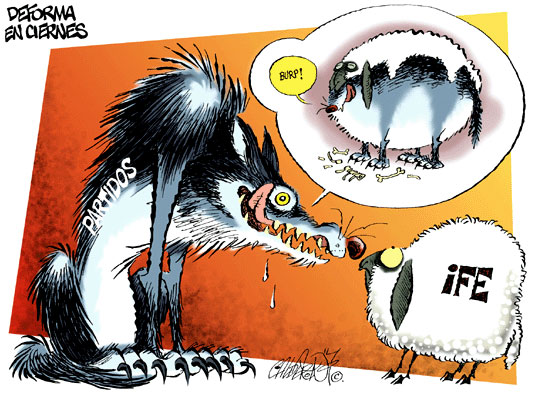
\includegraphics[width=\textwidth]{../../pics/calderonIFE20070829.jpg}

}
%%%%%%%%%%%%%%%%%%%%%%%%%%%%%%%%%%%%%%%%%%%%%%%%%%%%%%%%%%%%%%%%%%%%%%%%%%%%%%%%%%%%%%%%%%%%%%%% 
\frame {                      % SLIDE

    \frametitle{Our work on IFE, now and then}

\textbf{Before}: static ideal point estimation 1996--2007 \\
(Est\'evez, Magar, and Rosas 2008)

\begin{itemize}

\item Party watchdog model: expect party segmentation of Council General (same-sponsor councilors align).

\end{itemize}

\bigskip

\textbf{Now}: dynamic estimation 1996--2011

\begin{itemize}

\item Same general hypothesis, finer tests.

\item Longitudinal estimates: track realignment, effect of new
entrants, compare electoral semesters/rest...

\item Link dynamics to analytical narratives.

\end{itemize}

}
%%%%%%%%%%%%%%%%%%%%%%%%%%%%%%%%%%%%%%%%%%%%%%%%%%%%%%%%%%%%%%%%%%%%%%%%%%%%%%%%%%%%%%%%%%%%%%%%
% %\section{Outline}

% \frame {                      % SLIDE

%     \frametitle{Outline}

% \tableofcontents[section=1]

% }
%%%%%%%%%%%%%%%%%%%%%%%%%%%%%%%%%%%%%%%%%%%%%%%%%%%%%%%%%%%%%%%%%%%%%%%%%%%%%%%%%%%%%%%%%%%%%%%%
%\section{IFE and delegation}
\frame {                      % SLIDE

    \frametitle{The Federal Electoral Institute}

\begin{itemize}

\item Nine-member, non-partisan regulatory board

\item Decisions affect all aspects of party life

    \begin{enumerate}
        \item party finance
        \item candidate selection
        \item campaign contents
        \item leaders v.\ rank-and-file
        \item vote count
        \item ...
    \end{enumerate}

\item Congress appoints members (super-majority) for 7-year terms. Party quota/veto system (informal)

\item Public roll call votes

\end{itemize}

}
%%%%%%%%%%%%%%%%%%%%%%%%%%%%%%%%%%%%%%%%%%%%%%%%%%%%%%%%%%%%%%%%%%%%%%%%%%%%%%%%%%%%%%%%%%%%%%%%
\frame {                      % SLIDE

    \frametitle{Our argument}

\alert{Parties} designed election referee that they can influence

\bigskip

Delegation dilemmas: \\ IFE (the agent) affects parties'
(the principal) welfare

\bigskip

\begin{center}
Careful delegation $\rightarrow$ \alert{party} trust $\rightarrow$
citizen trust
\end{center}

\begin{block}{Contract design (Kiewiet \& McCubbins 1991)}
 \begin{center}
    \begin{itemize}
        \item screening
        \item monitoring
        \item rewards and sanctions
        \item checks and balances
    \end{itemize}
 \end{center}
\end{block}

%Collective principal raises additional complications

}
%%%%%%%%%%%%%%%%%%%%%%%%%%%%%%%%%%%%%%%%%%%%%%%%%%%%%%%%%%%%%%%%%%%%%%%%%%%%%%%%%%%%%%%%%%%%%%%%
%\section{Data and methods}

% \frame {                      % SLIDE

%     \frametitle{Stochastic spatial voting}

% \begin{center}
%  \begin{tikzpicture}[scale=1,rotate=0]
%   \def\xo{0,0}
%   \def\xu{4,0}
%   \def\xj{2.7,0}
%   \def\m{2,0}
%   \draw (-1,0) -- (5,0);
%   \fill[red] (\xo) circle (1.5pt) node [below=2pt,black] {$nay$};
%   \fill[green] (\xu) circle (1.5pt) node [below=2pt,black] {$aye$};
% %  \fill[black] (\xj) circle (1.5pt) node [below=2pt,black] {$x_j$};
%   \draw (2,.1) -- (2,-.1) node [below=2pt,black] {$m$};
% %  \fill[black!50] (\xj) circle (1.5pt) node [below=2pt,black] {$j$};
%  \end{tikzpicture}
% \end{center}

% \bigskip

% {\color{black!15}

% Vote propensity: $y^*_{j}= \delta(x_j - m) +\text{error}$.

% \bigskip

% Voting is sincere: $y_j=
%  \begin{cases}
%   1 \text{ (`aye')} \iff y^*_{j} \geq 0 \\
%   0 \text{ (`nay') otherwise.}           \,
%  \end{cases}$

% \bigskip

% Dynamics: $x_{j,t} \sim \mathrm{N}( x_{j,t-1},\text{slack}
% )$~~~~~(cf.\ Martin\&Quinn 2002).

% \bigskip

% Small assembly: Bayesian estimation via MCMC simulation. }

% }
%%%%%%%%%%%%%%%%%%%%%%%%%%%%%%%%%%%%%%%%%%%%%%%%%%%%%%%%%%%%%%%%%%%%%%%%%%%%%%%%%%%%%%%%%%%%%%%%

\frame {                      % SLIDE

    \frametitle{Stochastic spatial voting}

\begin{center}
 \begin{tikzpicture}[scale=1,rotate=0]
  \def\xo{0,0}
  \def\xu{4,0}
  \def\xj{2.7,0}
  \def\m{2,0}
  \draw (-1,0) -- (5,0);
  \fill[red] (\xo) circle (1.5pt) node [below=2pt,black] {$nay$};
  \fill[green] (\xu) circle (1.5pt) node [below=2pt,black] {$aye$};
  \fill[black] (\xj) circle (1.5pt) node [below=2pt,black] {$x_j$};
  \draw (2,.1) -- (2,-.1) node [below=2pt,black] {$m$};
%  \fill[black!50] (\xj) circle (1.5pt) node [below=2pt,black] {$j$};
 \end{tikzpicture}
\end{center}

\bigskip 

Vote propensity: $v^*_{j}= \texttt{signal}(x_j - m) +\texttt{error}$.

\bigskip 

Voting is sincere: $v_j=
 \begin{cases}
  1 \text{ (`aye')} \iff v^*_{j} \geq 0 \\
  0 \text{ (`nay') otherwise.}           \,
 \end{cases}$

\bigskip 

Small assembly: Bayesian estimation via MCMC simulation.

}
%%%%%%%%%%%%%%%%%%%%%%%%%%%%%%%%%%%%%%%%%%%%%%%%%%%%%%%%%%%%%%%%%%%%%%%%%%%%%%%%%%%%%%%%%%%%%%%%
\frame {                      % SLIDE

    \frametitle{Dynamics}
\bigskip 

Approach 1---Martin\&Quinn (2002): 

\begin{itemize}

\item For \alert{quarter} $t$: $x_{j,t} \sim \mathrm{N}( x_{j,t-1},\text{slack})$

\item \emph{Drawback}: votes vary considerably across quarters---ideal points sensitive to sheer volume of information (Desposato), so drift may be spurious 

\end{itemize}

\bigskip

Approach 2---Bonica (2010): 

\begin{itemize}

\item Allow estimates to vary over periods of very short duration: item $i \pm k$, $k=15$

\item \alert{Vote-by-vote} estimation

\item Periods mostly overlap, constraining short-term shifts 

\item IRT instead of OC

\end{itemize}

}
% %%%%%%%%%%%%%%%%%%%%%%%%%%%%%%%%%%%%%%%%%%%%%%%%%%%%%%%%%%%%%%%%%%%%%%%%%%%%%%%%%%%%%%%%%%%%%%%%
% \frame {                      % SLIDE

%     \frametitle{Meaning of recovered ideal points?}

% \begin{itemize}

% \item<2-> Poole \& Rosenthal: ideology.

% \item<3-> Literal interpretation valid only if intervening factors (strategy, institutions) absent.

% \item<4-> But: hardly absent.

% \item<4-> More agnostic: ideal point summary of councilor's voting
% record vis-�-vis rest.

% \item<4-> Closeness = \alert{vote likeness}.

% \end{itemize}

% }
%%%%%%%%%%%%%%%%%%%%%%%%%%%%%%%%%%%%%%%%%%%%%%%%%%%%%%%%%%%%%%%%%%%%%%%%%%%%%%%%%%%%%%%%%%%%%%%%
\frame {                      % SLIDE
    \frametitle{Contested votes}

\begin{center}

Votes: 3,907 unanimous, 1,446 contested (27\%)

\bigskip

% \includegraphics[width=\textwidth]{c:/data/rollcall/ife_cg/graphs/all+divVotsSemestre.pdf}
 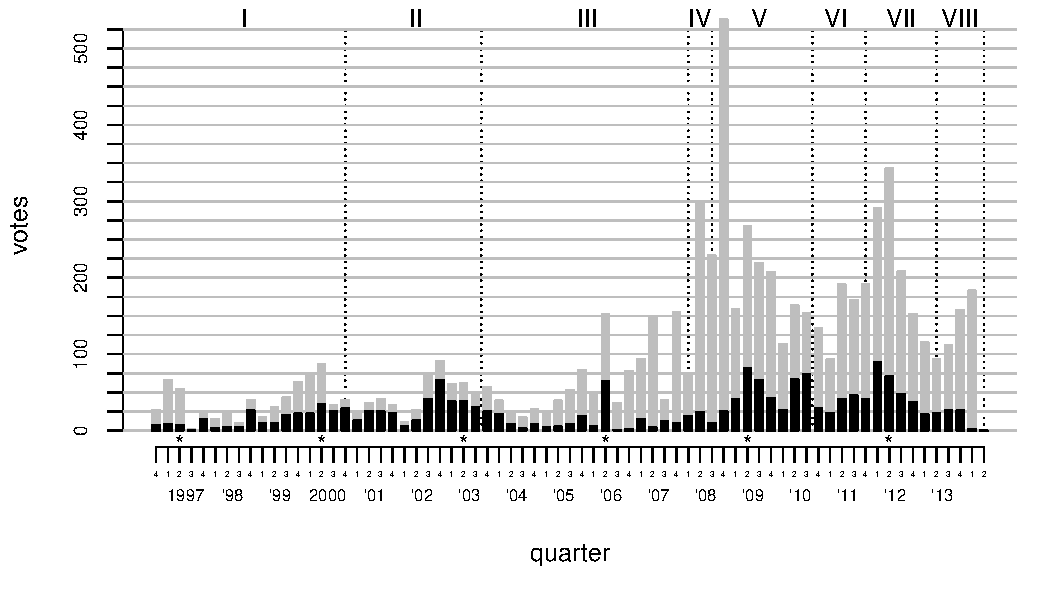
\includegraphics[width=\textwidth]{../../plots/all+divVotsQuarter.pdf}

\bigskip

%Presidents: Woldenberg (I--II); Ugalde (III); Vald\'es (IV--VII)
Same members within each period (I, II, ...) 

\end{center}

}
%%%%%%%%%%%%%%%%%%%%%%%%%%%%%%%%%%%%%%%%%%%%%%%%%%%%%%%%%%%%%%%%%%%%%%%%%%%%%%%%%%%%%%%%%%%%%%%%
%\section{Stability and change}
\frame {                      % SLIDE
    \frametitle{Results: 1996--2003 \textbf{quarterly}}

\begin{center}
% \includegraphics[width=.75\textwidth]{c:/data/rollcall/ife_cg/graphs/1dimDynWold9703jmayorPrecision.pdf} \\
 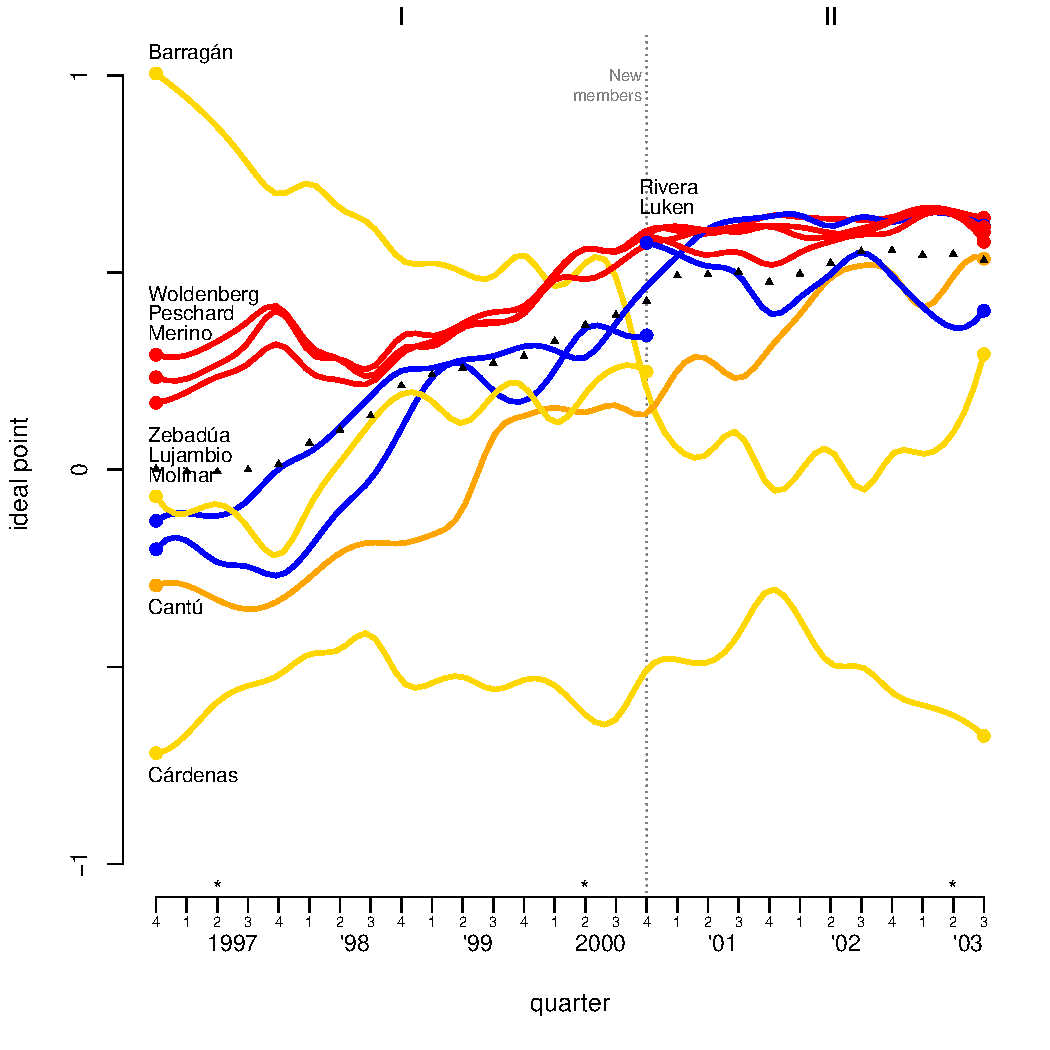
\includegraphics[width=.75\textwidth]{../../plots/lo-q-estuvo-compartido-c-memo/allWdynQuarter.pdf} \\
\end{center}

}
%%%%%%%%%%%%%%%%%%%%%%%%%%%%%%%%%%%%%%%%%%%%%%%%%%%%%%%%%%%%%%%%%%%%%%%%%%%%%%%%%%%%%%%%%%%%%%%%
\frame {                      % SLIDE
    \frametitle{Results: 1996--2003 \textbf{vote-by-vote}}

\begin{center}
 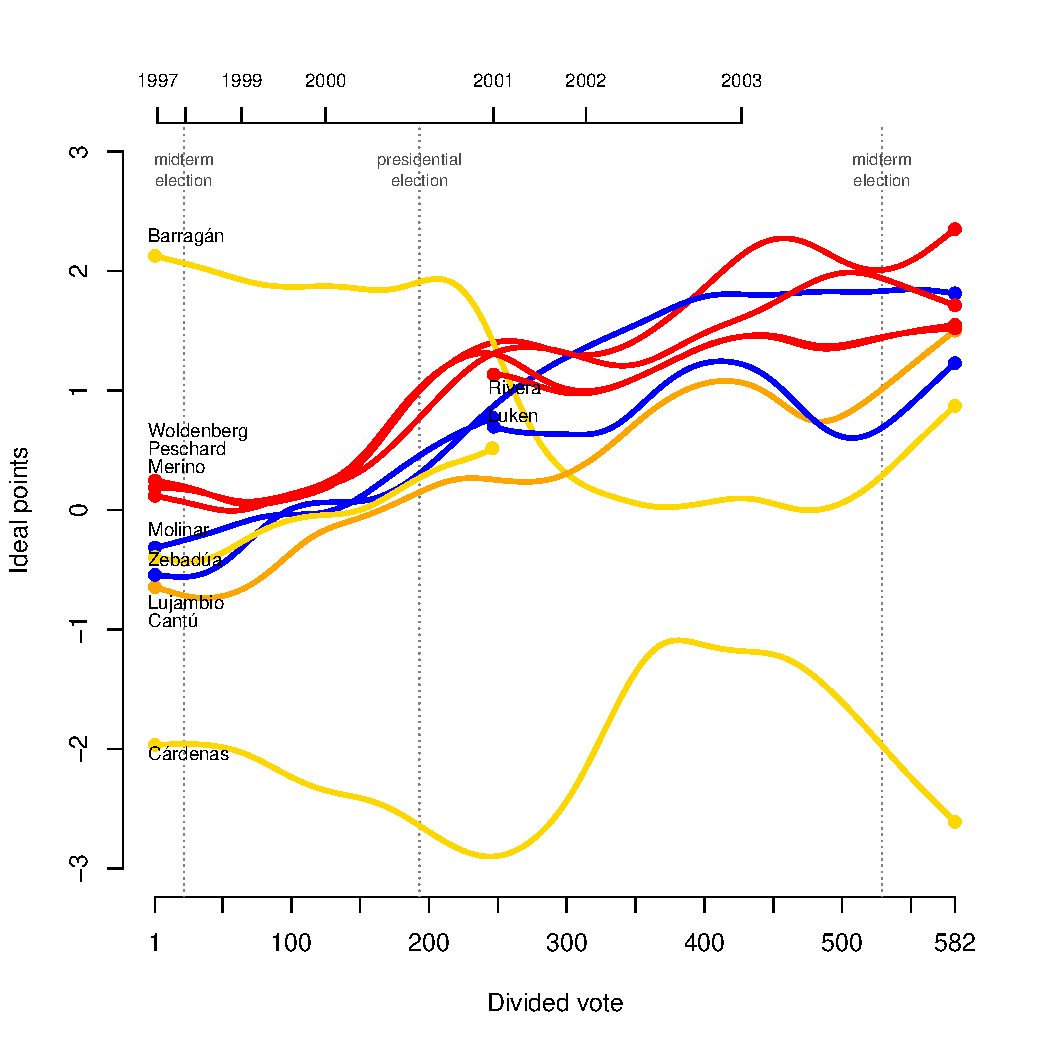
\includegraphics[width=.75\textwidth]{../../plots/lo-q-estuvo-compartido-c-memo/woldBonicaSmoothLines.pdf} \\
\end{center}

}
%%%%%%%%%%%%%%%%%%%%%%%%%%%%%%%%%%%%%%%%%%%%%%%%%%%%%%%%%%%%%%%%%%%%%%%%%%%%%%%%%%%%%%%%%%%%%%%%
\frame {                      % SLIDE
    \frametitle{Results: 2003--2011 \textbf{quarterly}}

\begin{center}
% \includegraphics[width=.75\textwidth]{c:/data/rollcall/ife_cg/graphs/1dimDynUgaVal0410j.pdf} \\
 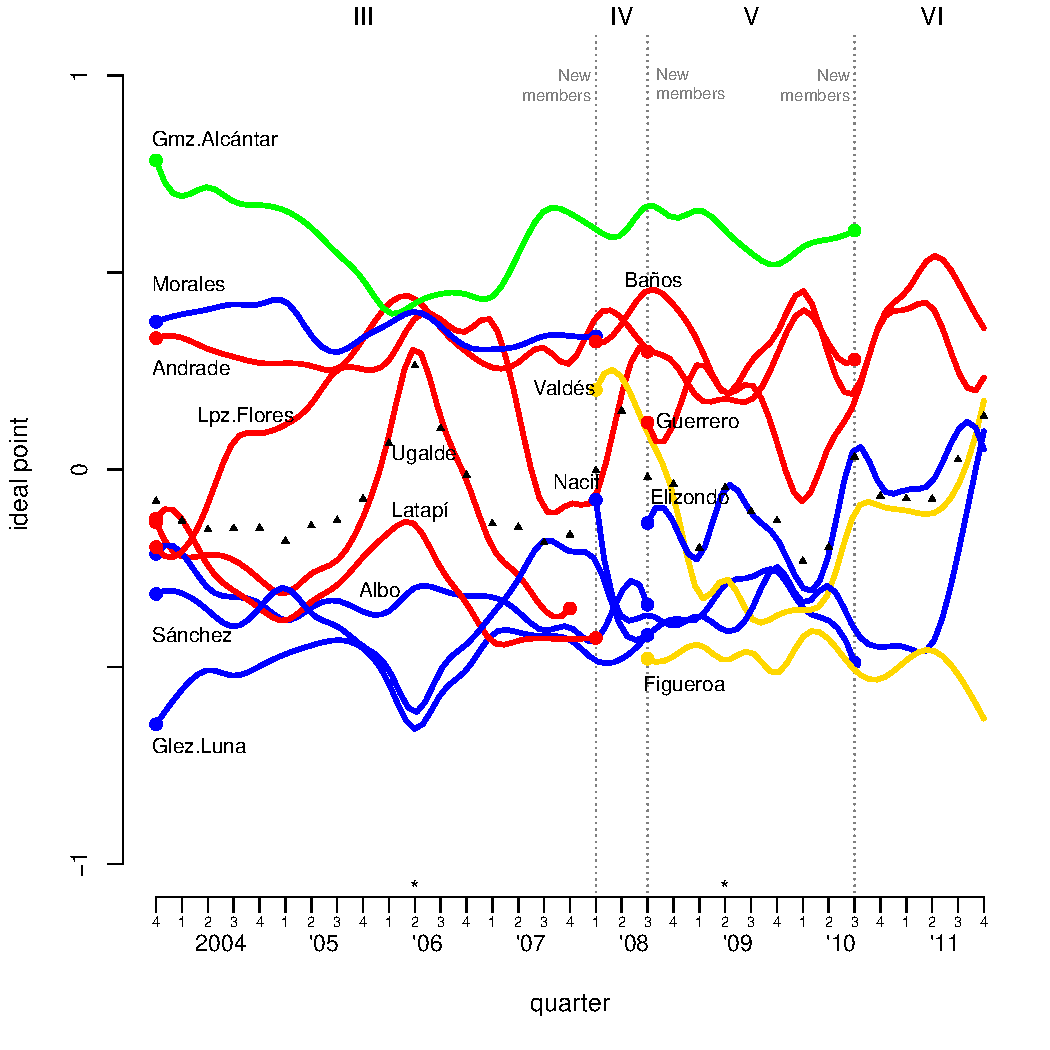
\includegraphics[width=.75\textwidth]{../../plots/lo-q-estuvo-compartido-c-memo/allUAVdynQuarter.pdf} \\
\end{center}
}
%%%%%%%%%%%%%%%%%%%%%%%%%%%%%%%%%%%%%%%%%%%%%%%%%%%%%%%%%%%%%%%%%%%%%%%%%%%%%%%%%%%%%%%%%%%%%%%%
%%\frame {                      % SLIDE
%%    \frametitle{Results}
%%
%%\begin{center}
%% \includegraphics[width=.75\textwidth]{c:/data/rollcall/ife_cg/graphs/allWpreW2dynNoNames.pdf} \\
%%\end{center}
%%
%%}
%%%%%%%%%%%%%%%%%%%%%%%%%%%%%%%%%%%%%%%%%%%%%%%%%%%%%%%%%%%%%%%%%%%%%%%%%%%%%%%%%%%%%%%%%%%%%%%%%%
%%\frame {                      % SLIDE
%%    \frametitle{Results}
%%
%%\begin{center}
%% \includegraphics[width=.75\textwidth]{c:/data/rollcall/ife_cg/graphs/allWpreW2dyn.pdf} \\
%%\end{center}
%%
%%}
%%%%%%%%%%%%%%%%%%%%%%%%%%%%%%%%%%%%%%%%%%%%%%%%%%%%%%%%%%%%%%%%%%%%%%%%%%%%%%%%%%%%%%%%%%%%%%%%
\frame {                      % SLIDE

    \frametitle{What lies behind drift?}


\begin{tabular}{cll}
 & \emph{Type}                    & \emph{Effect on ideal points} \\ \hline
 1.&Screening   & Concomitant shifts among  \\
   &                       & same-sponsor councilors \\
 2.&Constituent pressure & Shifts should \emph{follow} change in principal's \\
   &                       & situation (eg.\ new Congress) \\
 3.&Gatekeeping            & Removal of divisive issues pulls \\
   &                       & most together \\ \hline
 % 3.&Sophisticated voting   & Moderates change sides \\
 % 4.&Side payments          & Moderates shift towards those \\
 %   &                       & trading with \\ \hline
\end{tabular}

}
%%%%%%%%%%%%%%%%%%%%%%%%%%%%%%%%%%%%%%%%%%%%%%%%%%%%%%%%%%%%%%%%%%%%%%%%%%%%%%%%%%%%%%%%%%%%%%%% 
\frame {                      % SLIDE

    \frametitle{Some empirical indicators}

 \begin{enumerate}
  \item New Congress = new principal
  \item Congressional party split = two new principals
  \item Election quarters = less agenda control by IFE (party complaints)
 \end{enumerate}


\begin{block}{Party complaints filed as \% of all votes}
 \begin{center}
  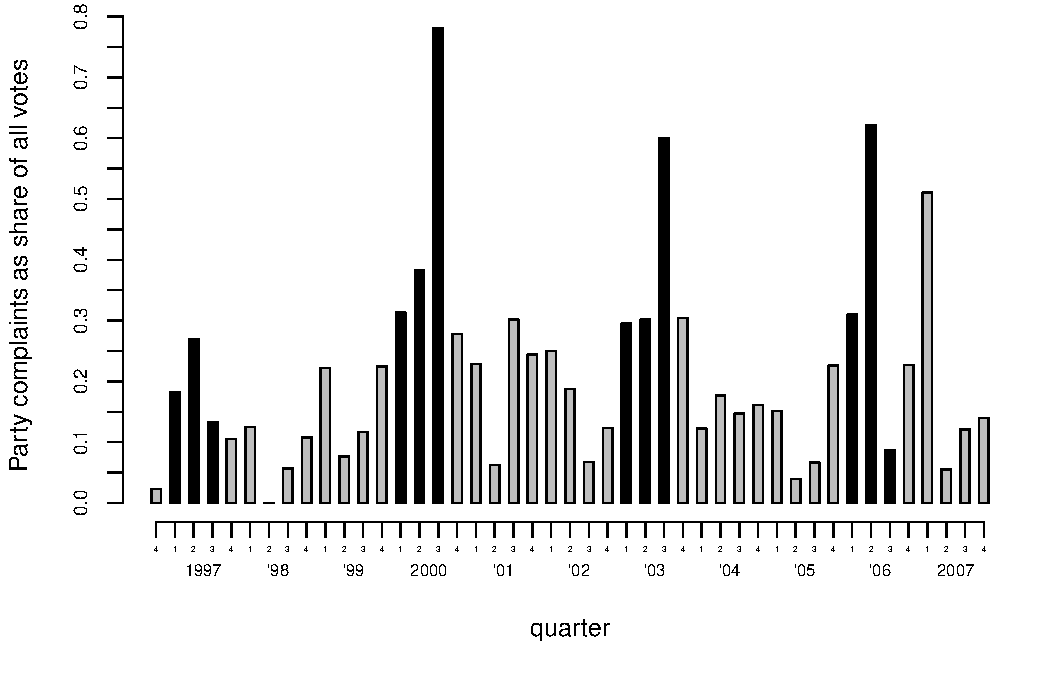
\includegraphics[width=.7\textwidth]{../../plots/lo-q-estuvo-compartido-c-memo/sharePtyComplaintsQuarter.pdf}
 \end{center}
\end{block}

}
%%%%%%%%%%%%%%%%%%%%%%%%%%%%%%%%%%%%%%%%%%%%%%%%%%%%%%%%%%%%%%%%%%%%%%%%%%%%%%%%%%%%%%%%%%%%%%%%%
\frame {                      % SLIDE
    \frametitle{Results: overlapping}

\begin{center}
% \includegraphics[width=.75\textwidth]{c:/data/rollcall/ife_cg/graphs/woStackPRI.pdf} \\
 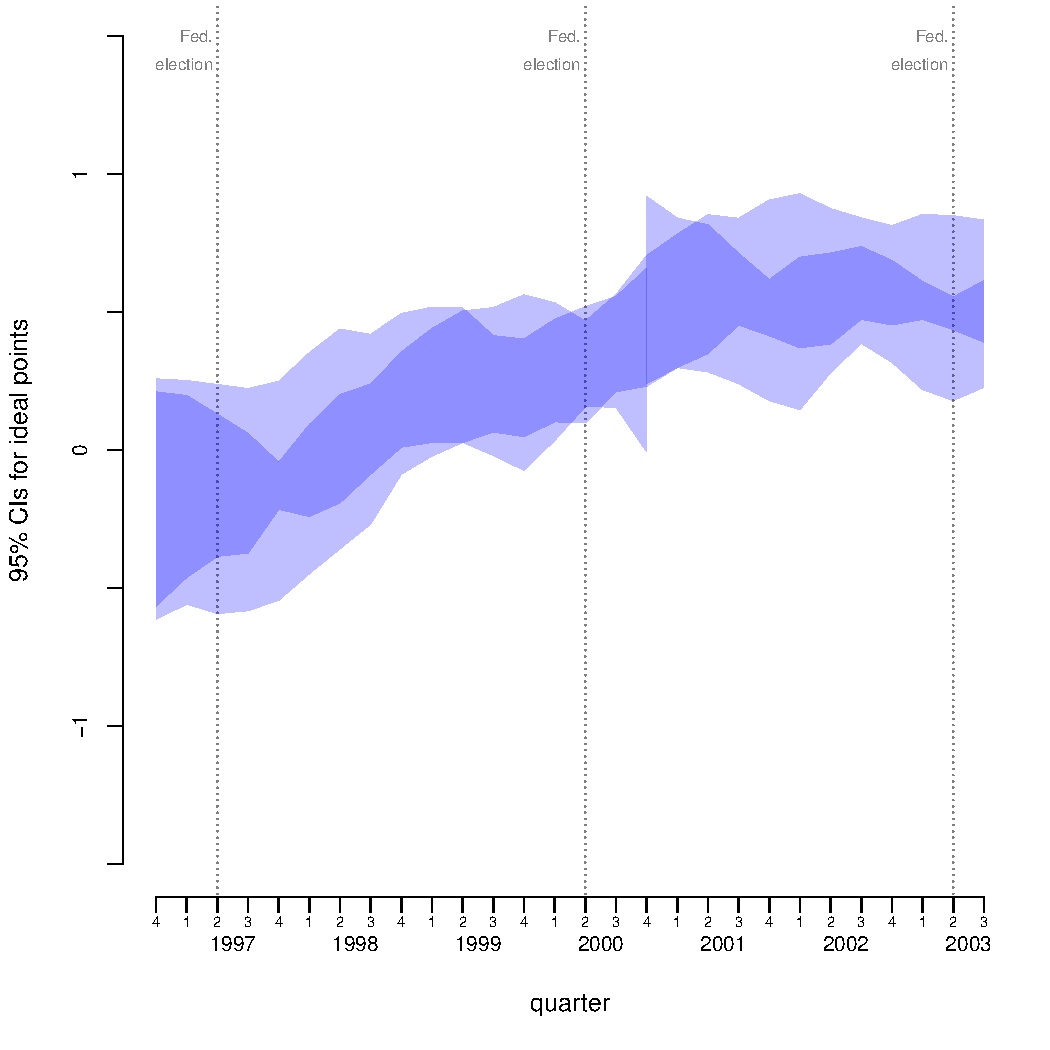
\includegraphics[width=.75\textwidth]{../../plots/lo-q-estuvo-compartido-c-memo/woldStackMartinQuinnQuarterPan.pdf} \\
\end{center}

}
%%%%%%%%%%%%%%%%%%%%%%%%%%%%%%%%%%%%%%%%%%%%%%%%%%%%%%%%%%%%%%%%%%%%%%%%%%%%%%%%%%%%%%%%%%%%%%%%
\frame {                      % SLIDE
    \frametitle{Results: overlapping}

\begin{center}
 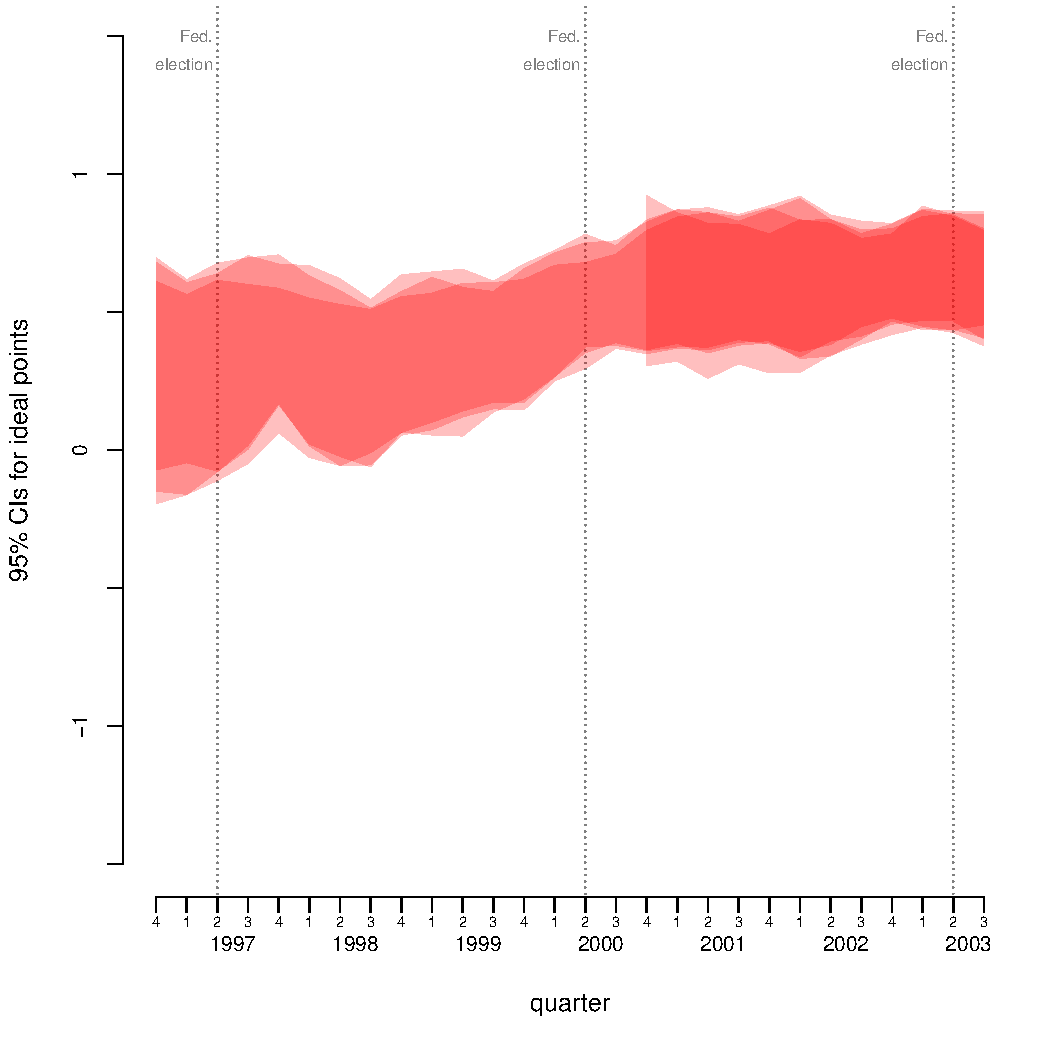
\includegraphics[width=.75\textwidth]{../../plots/lo-q-estuvo-compartido-c-memo/woldStackMartinQuinnQuarterPri.pdf} \\
\end{center}
}
%%%%%%%%%%%%%%%%%%%%%%%%%%%%%%%%%%%%%%%%%%%%%%%%%%%%%%%%%%%%%%%%%%%%%%%%%%%%%%%%%%%%%%%%%%%%%%%%
\frame {                      % SLIDE
    \frametitle{Results: overlapping}

\begin{center}
 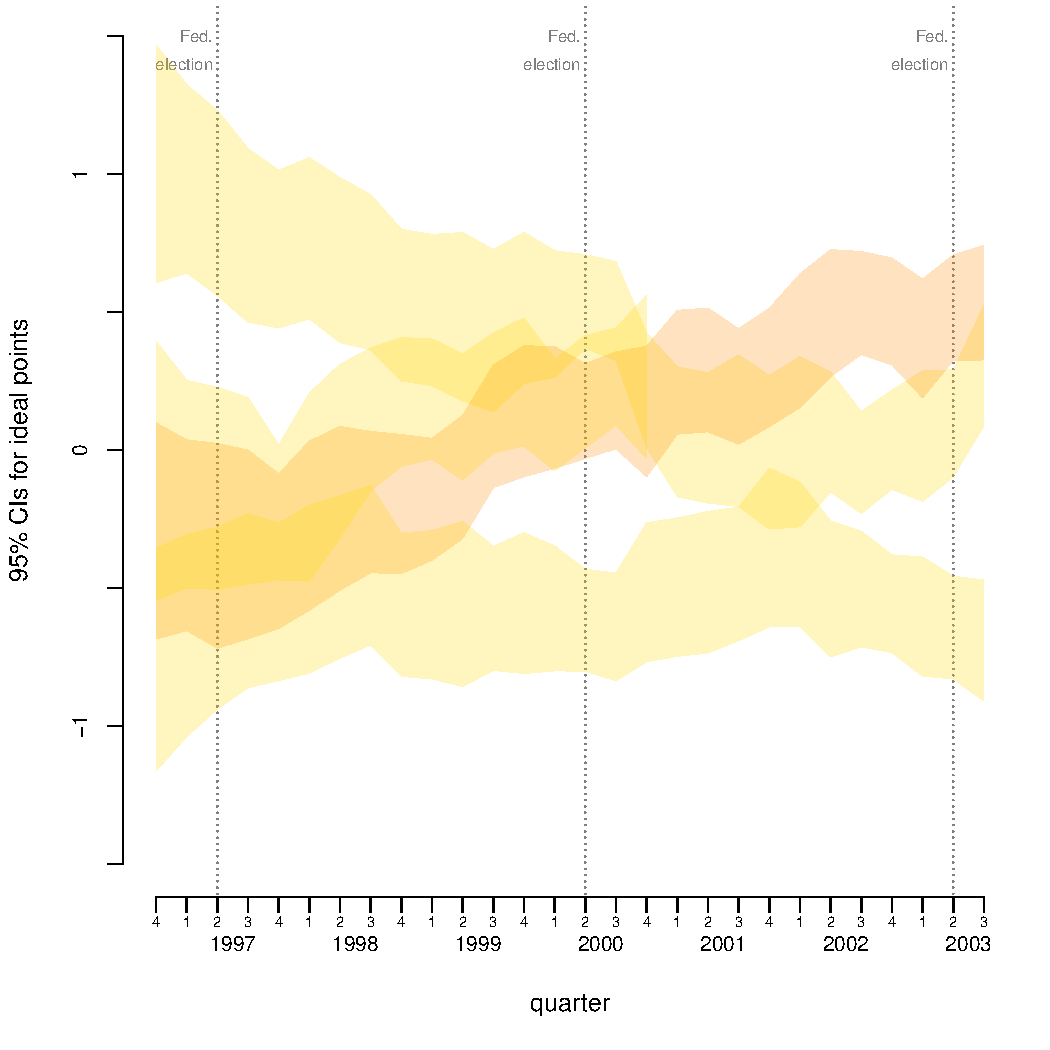
\includegraphics[width=.75\textwidth]{../../plots/lo-q-estuvo-compartido-c-memo/woldStackMartinQuinnQuarterLeft.pdf} \\
\end{center}
}
%%%%%%%%%%%%%%%%%%%%%%%%%%%%%%%%%%%%%%%%%%%%%%%%%%%%%%%%%%%%%%%%%%%%%%%%%%%%%%%%%%%%%%%%%%%%%%%%
\frame {                      % SLIDE
    \frametitle{Results: overlap in two models}

\begin{center}
  \begin{tabular}{ccc}
    \multicolumn{3}{c}{} \\
%    (a) Vote-by-vote & (b) Vote-by-vote & (c) Vote-by-vote\\
%    PAN & PRI & Left\\
    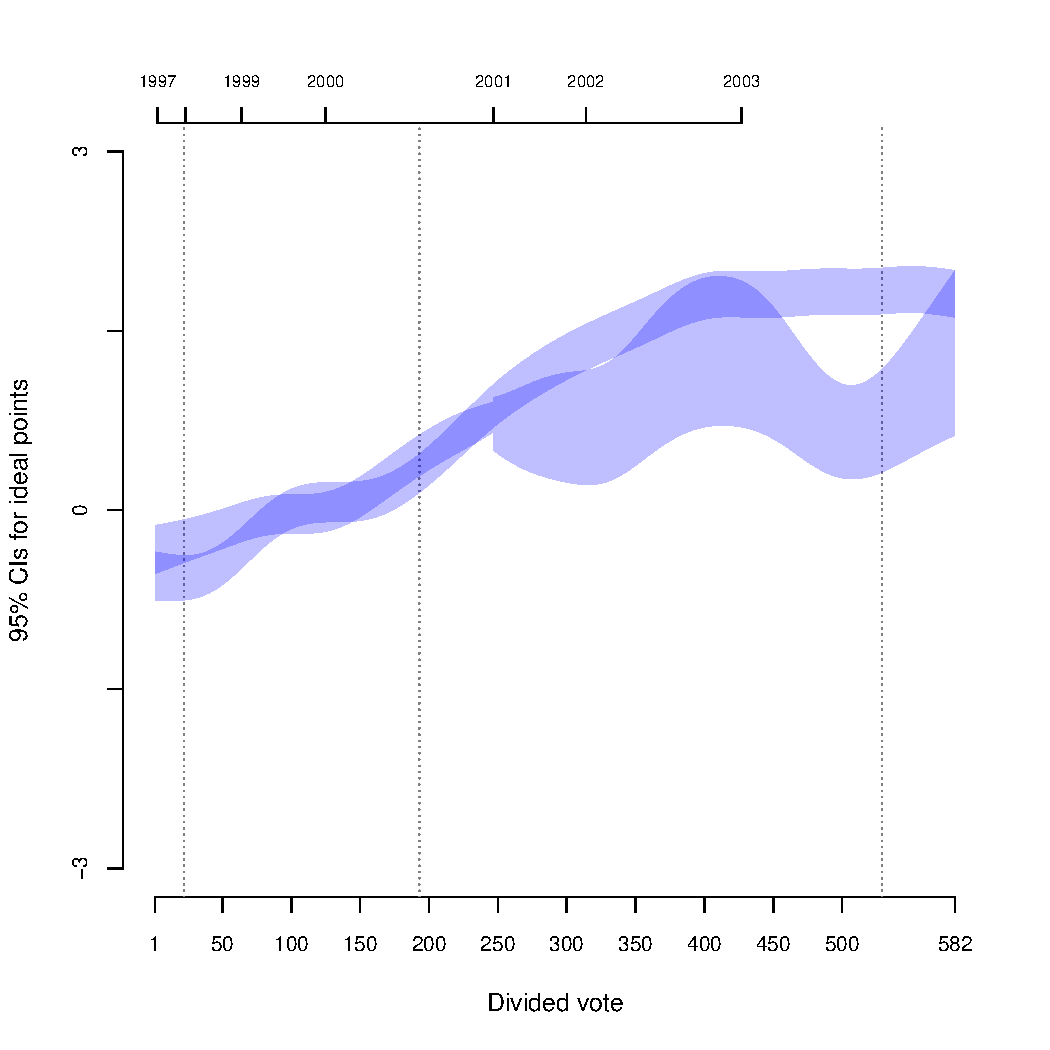
\includegraphics[width=.3\textwidth]{../../plots/lo-q-estuvo-compartido-c-memo/woldStackBonicaPan.pdf} &
    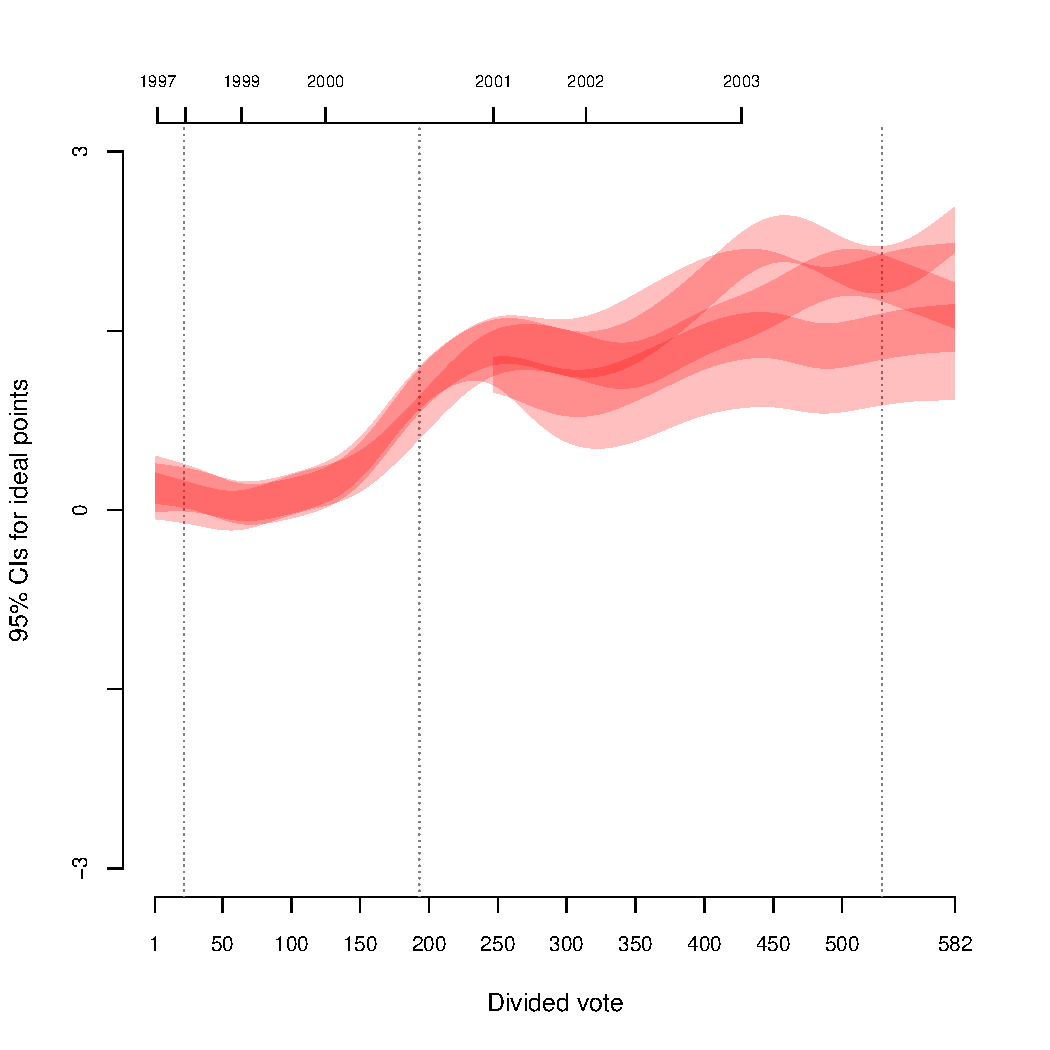
\includegraphics[width=.3\textwidth]{../../plots/lo-q-estuvo-compartido-c-memo/woldStackBonicaPri.pdf} &
    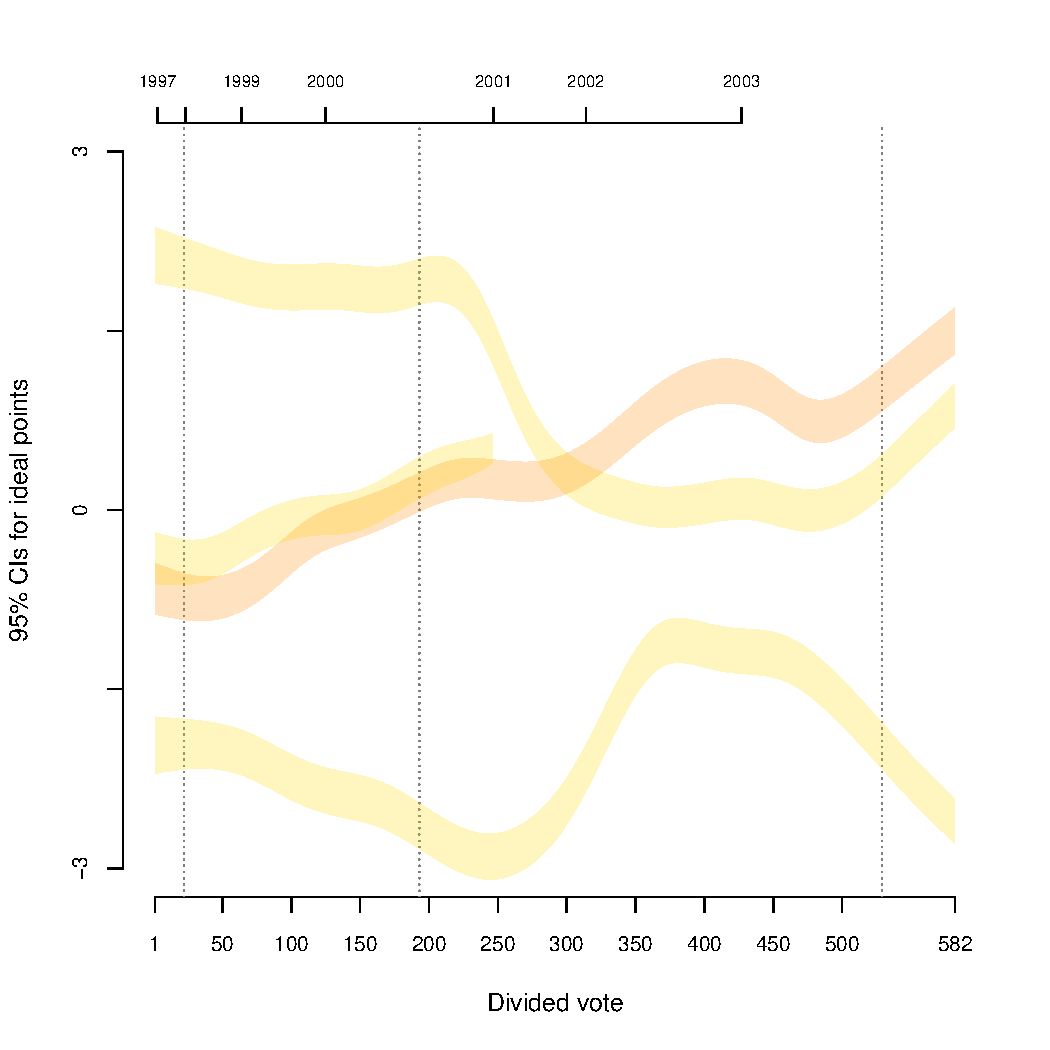
\includegraphics[width=.3\textwidth]{../../plots/lo-q-estuvo-compartido-c-memo/woldStackBonicaLeft.pdf} \\
    \multicolumn{3}{c}{} \\
%    (d) Quarter-by-quarter & (e) Quarter-by-quarter & (f) Quarter-by-quarter\\
%    PAN & PRI & Left \\
    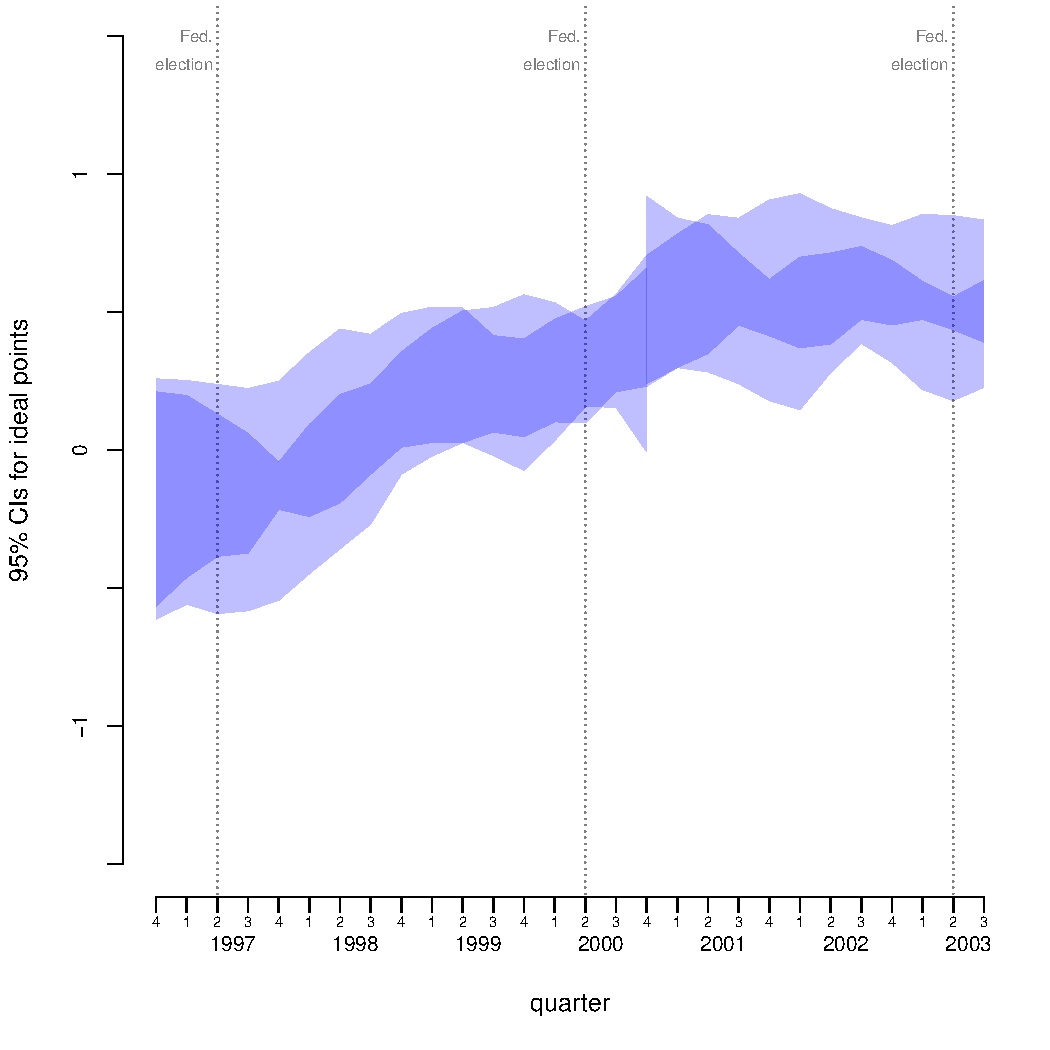
\includegraphics[width=.3\textwidth]{../../plots/lo-q-estuvo-compartido-c-memo/woldStackMartinQuinnQuarterPan.pdf} &
    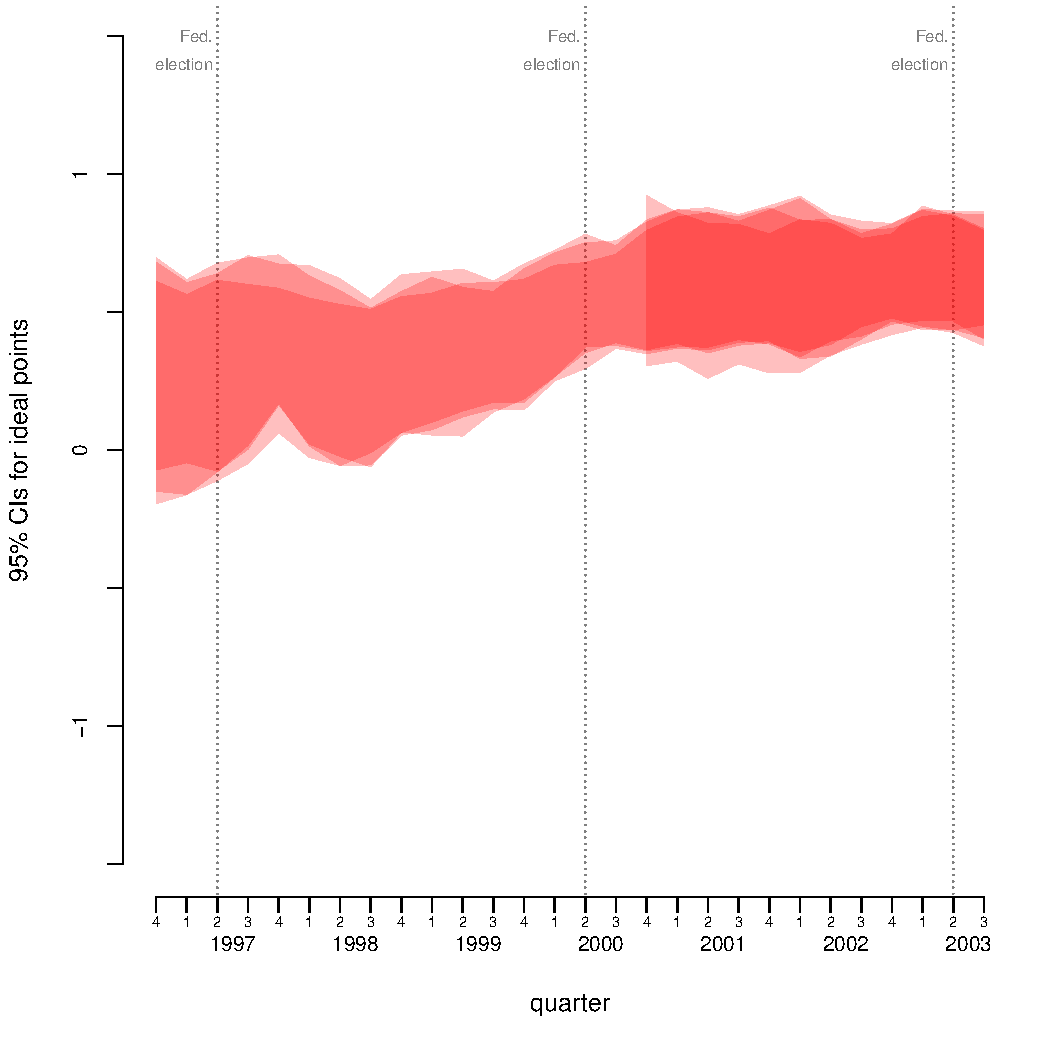
\includegraphics[width=.3\textwidth]{../../plots/lo-q-estuvo-compartido-c-memo/woldStackMartinQuinnQuarterPri.pdf} &
    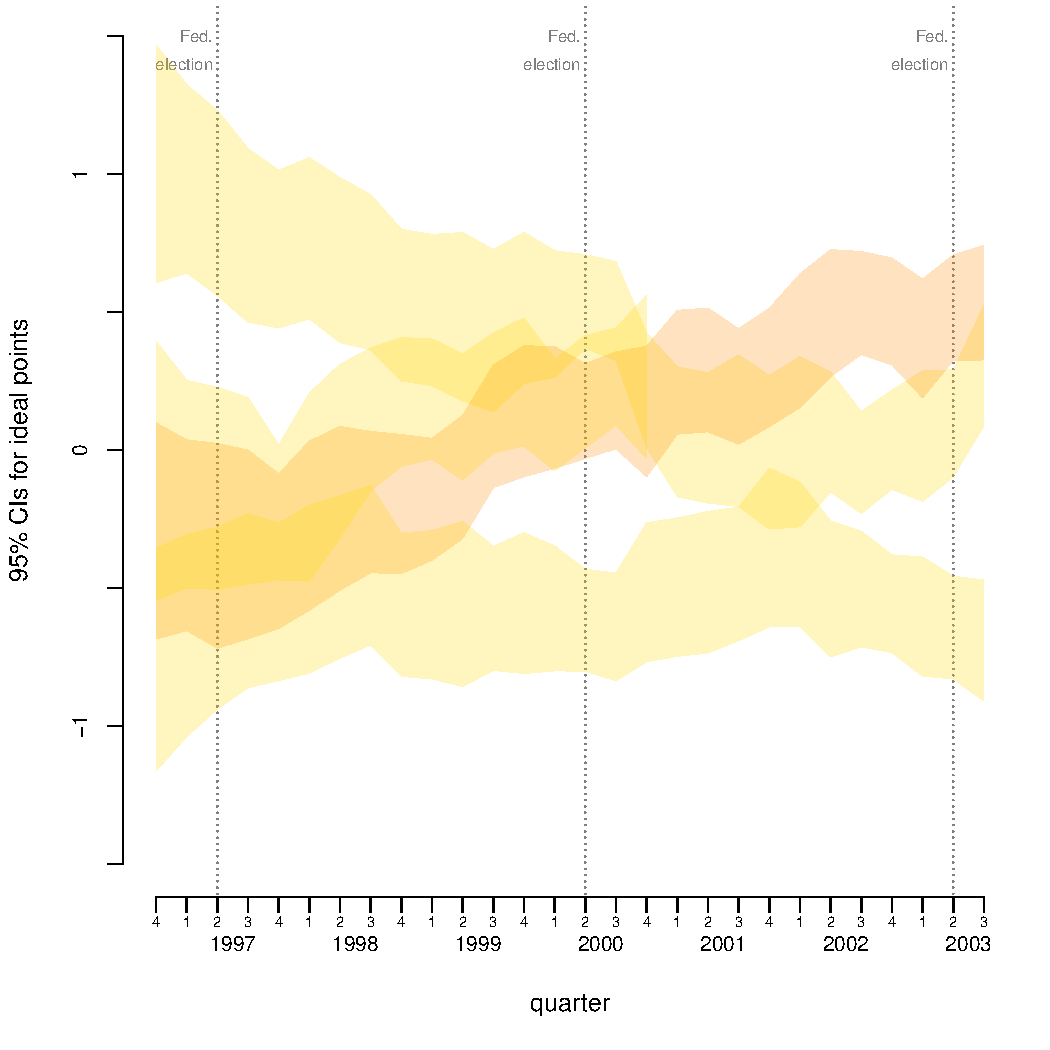
\includegraphics[width=.3\textwidth]{../../plots/lo-q-estuvo-compartido-c-memo/woldStackMartinQuinnQuarterLeft.pdf} \\
  \end{tabular}
\end{center}

}
%%%%%%%%%%%%%%%%%%%%%%%%%%%%%%%%%%%%%%%%%%%%%%%%%%%%%%%%%%%%%%%%%%%%%%%%%%%%%%%%%%%%%%%%%%%%%%%%
\frame {                      % SLIDE
    \frametitle{Results: overlapping}

\begin{center}
 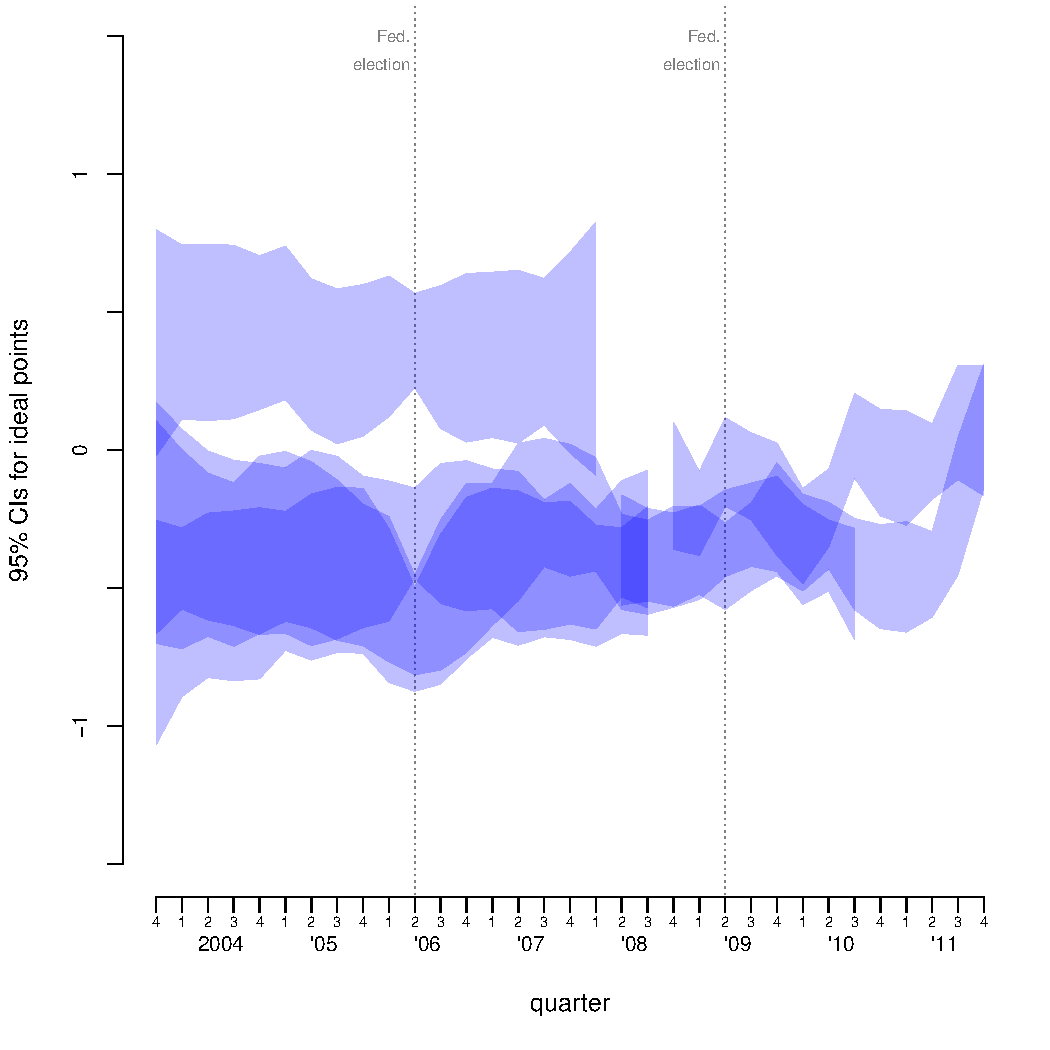
\includegraphics[width=.75\textwidth]{../../plots/lo-q-estuvo-compartido-c-memo/uavStackMartinQuinnQuarterPan.pdf} \\
\end{center}

}
%%%%%%%%%%%%%%%%%%%%%%%%%%%%%%%%%%%%%%%%%%%%%%%%%%%%%%%%%%%%%%%%%%%%%%%%%%%%%%%%%%%%%%%%%%%%%%%%
\frame {                      % SLIDE
    \frametitle{Results: overlapping}

\begin{center}
 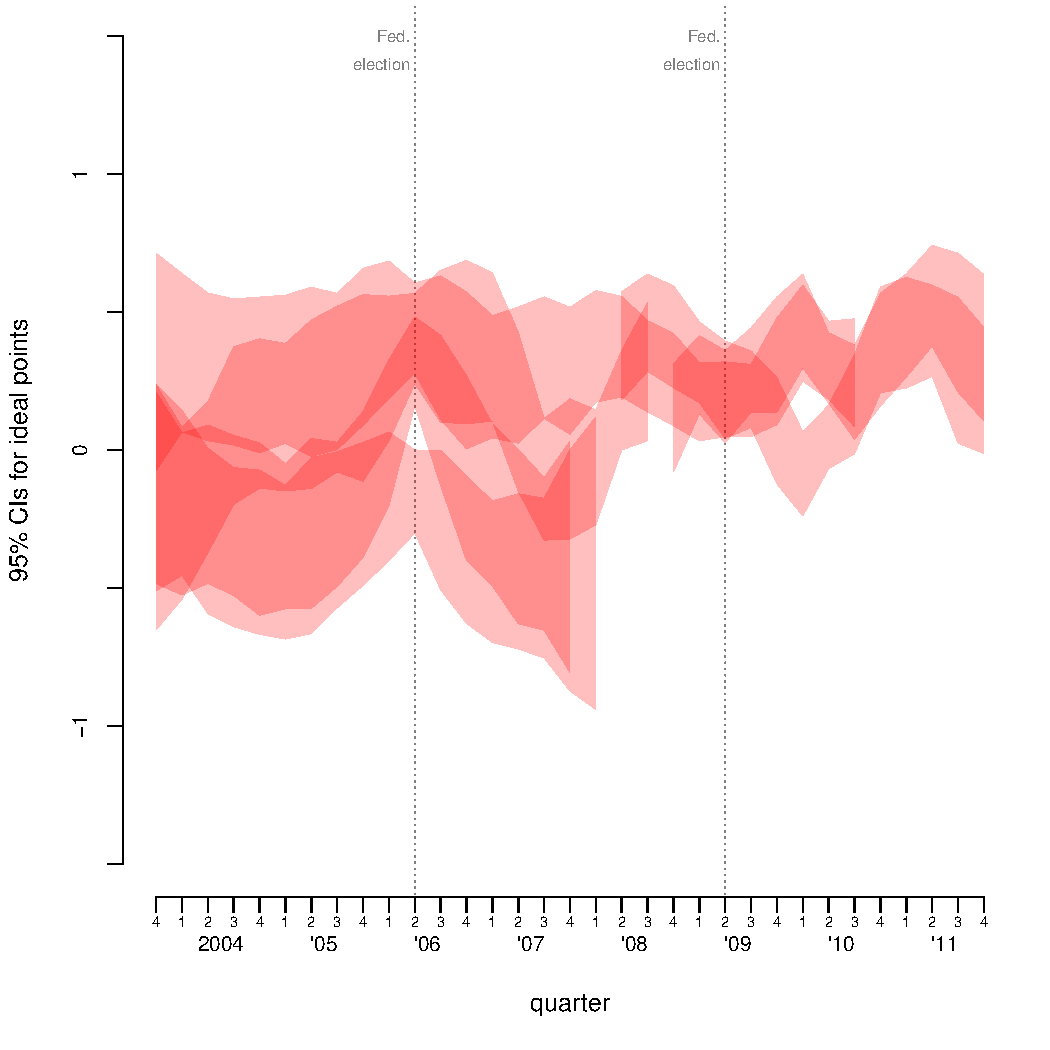
\includegraphics[width=.75\textwidth]{../../plots/lo-q-estuvo-compartido-c-memo/uavStackMartinQuinnQuarterPri.pdf} \\
\end{center}

}
%%%%%%%%%%%%%%%%%%%%%%%%%%%%%%%%%%%%%%%%%%%%%%%%%%%%%%%%%%%%%%%%%%%%%%%%%%%%%%%%%%%%%%%%%%%%%%%%
\frame {                      % SLIDE
    \frametitle{Results: overlapping}

\begin{center}
 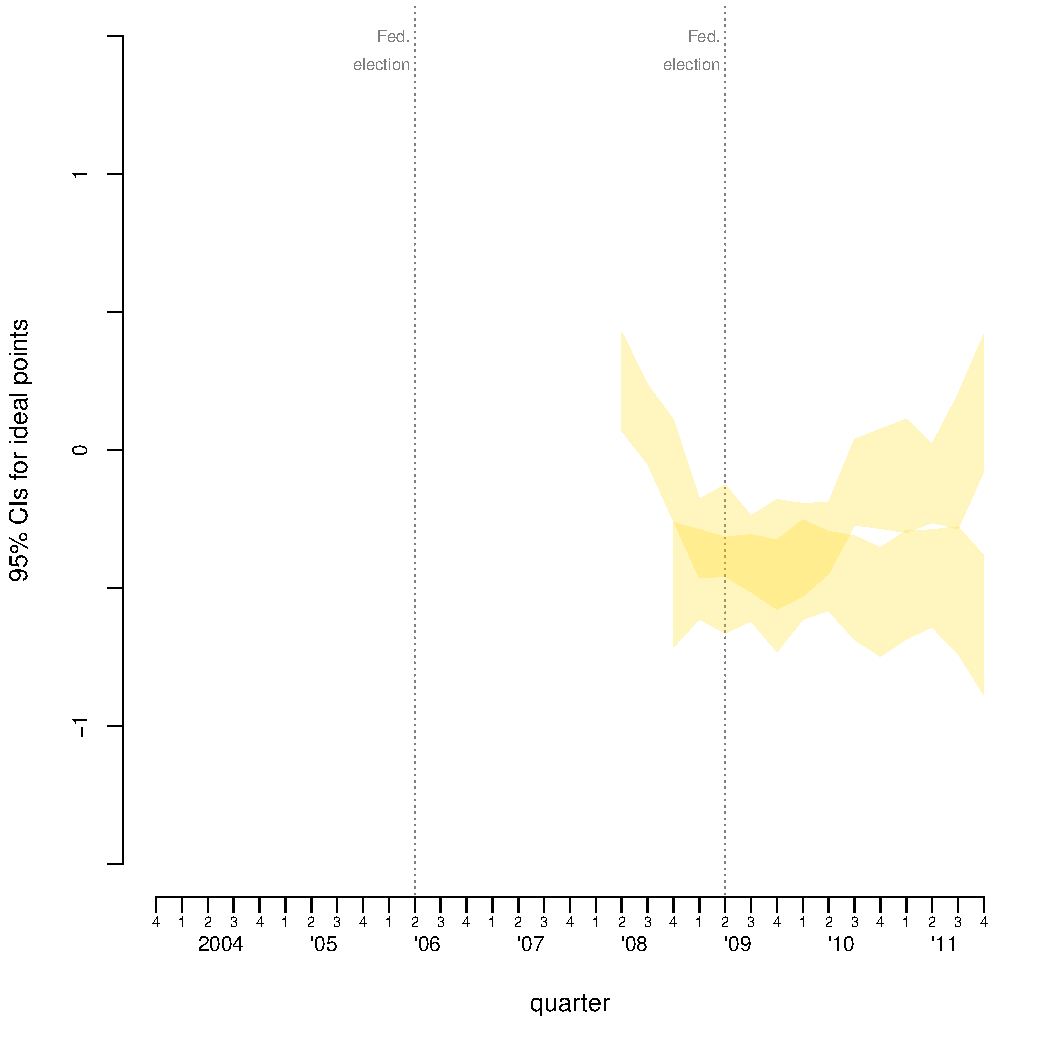
\includegraphics[width=.75\textwidth]{../../plots/lo-q-estuvo-compartido-c-memo/uavStackMartinQuinnQuarterLeft.pdf} \\
\end{center}

}
%%%%%%%%%%%%%%%%%%%%%%%%%%%%%%%%%%%%%%%%%%%%%%%%%%%%%%%%%%%%%%%%%%%%%%%%%%%%%%%%%%%%%%%%%%%%%%%%
\frame {                      % SLIDE
    \frametitle{Results: overlapping}

\begin{center}
 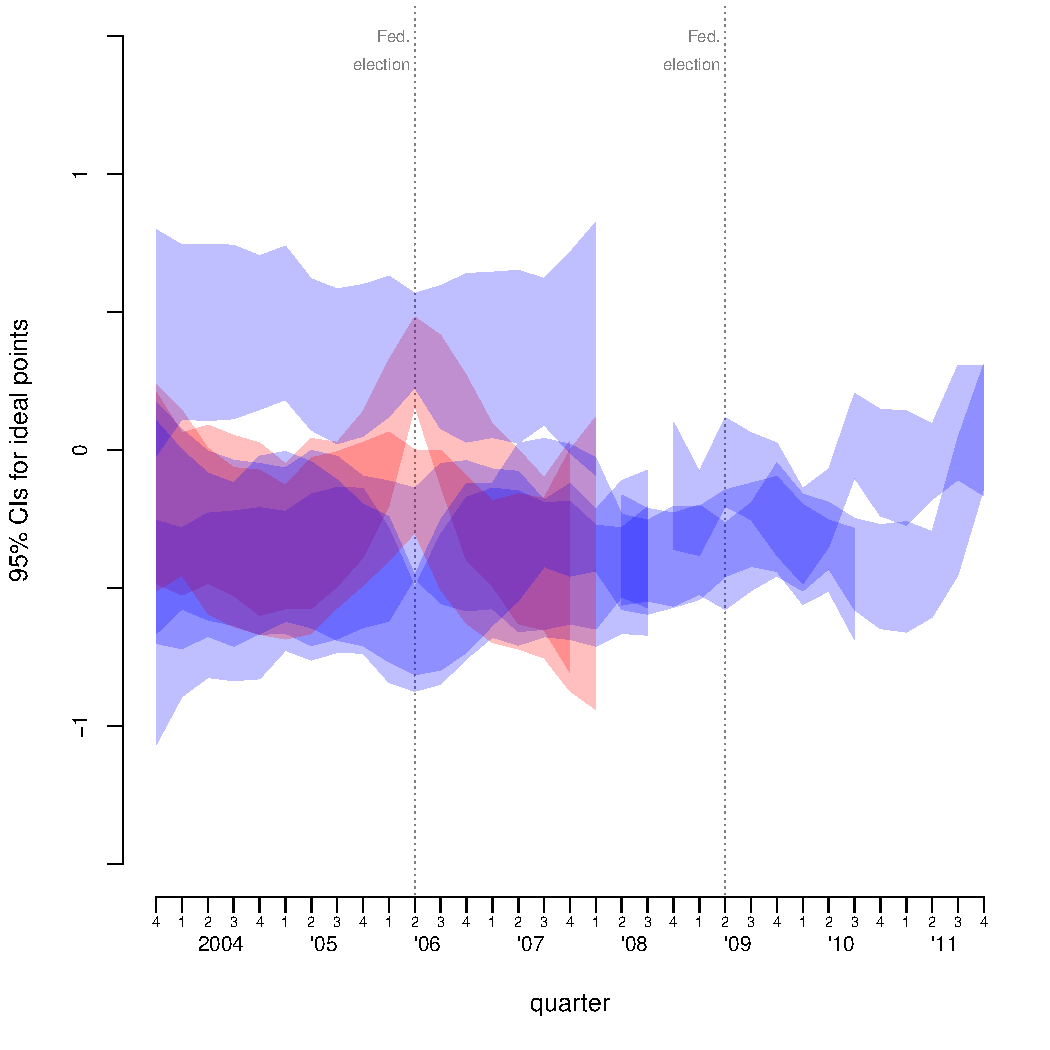
\includegraphics[width=.75\textwidth]{../../plots/lo-q-estuvo-compartido-c-memo/uavStackMartinQuinnQuarterPanElba.pdf} \\
\end{center}

}
%%%%%%%%%%%%%%%%%%%%%%%%%%%%%%%%%%%%%%%%%%%%%%%%%%%%%%%%%%%%%%%%%%%%%%%%%%%%%%%%%%%%%%%%%%%%%%%%
\frame {                      % SLIDE
    \frametitle{Results: overlapping}

\begin{center}
 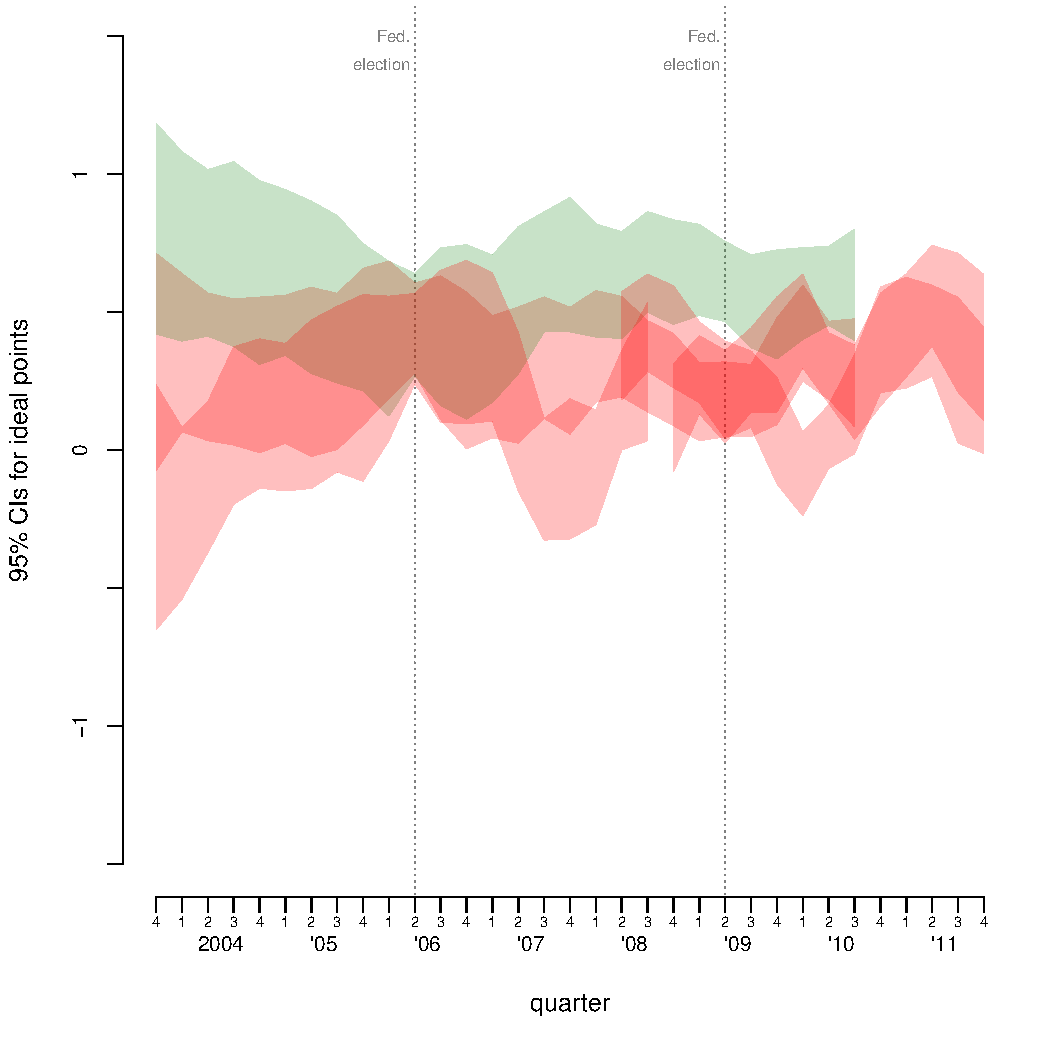
\includegraphics[width=.75\textwidth]{../../plots/lo-q-estuvo-compartido-c-memo/uavStackMartinQuinnQuarterPriMadPvem.pdf} \\
\end{center}

}
%%%%%%%%%%%%%%%%%%%%%%%%%%%%%%%%%%%%%%%%%%%%%%%%%%%%%%%%%%%%%%%%%%%%%%%%%%%%%%%%%%%%%%%%%%%%%%%%

\frame {                      % SLIDE

    \frametitle{New principal and inter-quarter change}

 \begin{center}
   \begin{tabular}{clcc}
    \multicolumn{2}{c}{Posterior $|x_{j,t+1}-x_{j,t}|$}&  Mean & Std.\ dev. \\ \hline
    a& New Congress quarters  & \alert{.140}  &   .115    \\
    b& Rest                   & \alert{.108}  &   .084    \\
    c& Prob.\ a>b             & \multicolumn{2}{c}{.560} \\ \hline
   \end{tabular}
 \end{center}

}

%%%%%%%%%%%%%%%%%%%%%%%%%%%%%%%%%%%%%%%%%%%%%%%%%%%%%%%%%%%%%%%%%%%%%%%%%%%%%%%%%%%%%%%%%%%%%%%%

\frame {                      % SLIDE

    \frametitle{Gatekeeping and signal-to-noise ratio}

 \begin{center}

   \begin{tabular}{clcc}
    \multicolumn{2}{c}{Posterior $|\texttt{signal}_i|$} &  Mean & Std.\ dev. \\ \hline
    d& Electoral quarters     & \alert{2.677} & 1.682  \\
    e& Rest                   & \alert{2.601} & 1.684  \\
    f& Prob.\ d>e             & \multicolumn{2}{c}{.565} \\ \hline
   \end{tabular}

\bigskip
\bigskip

   \begin{tabular}{clcc}
    \multicolumn{4}{c}{Posterior  $\texttt{signal}_i$s with .95 ci off zero} \\ \hline
    g& Percentage electoral quarters  & \multicolumn{2}{c}{\alert{53\%}} \\
    h& Percentage rest                & \multicolumn{2}{c}{\alert{45\%}} \\ \hline
%    \multicolumn{4}{c}{Abstention rates}   \\
%    i& PAN electoral semester & 0.039 & 0.054  \\
%    j& PAN rest               & 0.046 & 0.067  \\
%    k& PRI electoral semester & 0.016 & 0.021  \\
%    l& PRI rest               & 0.024 & 0.012  \\
%    m& PRD electoral semester & 0.072 & 0.031  \\
%    n& PRD rest               & 0.153 & 0.050  \\ \hline
   \end{tabular}
 \end{center}

}
%% %%%%%%%%%%%%%%%%%%%%%%%%%%%%%%%%%%%%%%%%%%%%%%%%%%%%%%%%%%%%%%%%%%%%%%%%%%%%%%%%%%%%%%%%%%%%%%%% 
%% \frame {                      % SLIDE
%%     \frametitle{Elections and within-contingent cohesion}
%%
%%  \begin{center}
%%   \begin{tabular}{llrrrr}
%%                   &  & \multicolumn{2}{c}{Electoral} &  \multicolumn{2}{c}{Non-electoral} \\
%%                   &  & \multicolumn{2}{c}{semester}  &  \multicolumn{2}{c}{semester}      \\
%%                   &  & Mean      & Std.\ dev.        & Mean    & Std.\ dev.              \\ \hline
%%    PRI    &          &  0.462    & 0.422   &   0.324  &  0.287  \\
%%    PAN    &          &  0.650    & 0.310   &   0.679  &  0.330  \\
%%    PRD    &          &  0.979    & 0.183   &   1.120  &  0.230  \\ \hline
%%   \end{tabular}
%%  \end{center}
%%
%%
%% }
%% %%%%%%%%%%%%%%%%%%%%%%%%%%%%%%%%%%%%%%%%%%%%%%%%%%%%%%%%%%%%%%%%%%%%%%%%%%%%%%%%%%%%%%%%%%%%%%%%
%% \frame {                      % SLIDE
%%     \frametitle{Elections and contingent median polarization}
%%
%%  \begin{center}
%%   \begin{tabular}{llrrrr}
%%                   & \multicolumn{2}{c}{Electoral} &  \multicolumn{2}{c}{Non-electoral} \\
%%                   & \multicolumn{2}{c}{semester}  &  \multicolumn{2}{c}{semester}      \\
%%                   & Mean      & Std.\ dev.        & Mean    & Std.\ dev.              \\ \hline
%%    \multicolumn{5}{c}{Periods I and II}  \\
%%    PRI-PAN &  0.155    & 0.130   &   0.091  &  0.125  \\
%%    PRI-PRD &  0.417    & 0.139   &   0.413  &  0.152  \\
%%    PAN-PRD &  0.262    & 0.163   &   0.323  &  0.170  \\
%%    \multicolumn{5}{c}{Period III}  \\
%%    PRI-PAN & 0.639    & 0.140   &   0.369  &  0.160  \\
%%   \end{tabular}
%%  \end{center}
%%
%%
%% }
% %%%%%%%%%%%%%%%%%%%%%%%%%%%%%%%%%%%%%%%%%%%%%%%%%%%%%%%%%%%%%%%%%%%%%%%%%%%%%%%%%%%%%%%%%%%%%%%%
% \frame {                      % SLIDE
%     \frametitle{Elections and contingent median polarization}

%  \begin{center}
%   \begin{tabular}{lccc}
%                   & Electoral & & Non-electoral \\
%                   & semester  & & semester      \\
%                   & mean  &     & mean      \\
%                   & \multicolumn{3}{c}{Periods I and II}  \\
%    PRI-PAN &  0.155    & \textbf{>}   &   0.091      \\
%    PRI-PRD &  0.417    & \textbf{=}   &   0.413      \\
%    PAN-PRD &  0.262    & \textbf{<}   &   0.323      \\ \\
%                   & \multicolumn{3}{c}{Period III}  \\
%    PRI-PAN &  0.639    &  \textbf{>}  &   0.369      \\
%   \end{tabular}
%  \end{center}


% }
%%%%%%%%%%%%%%%%%%%%%%%%%%%%%%%%%%%%%%%%%%%%%%%%%%%%%%%%%%%%%%%%%%%%%%%%%%%%%%%%%%%%%%%%%%%%%%%%%
\frame {                      % SLIDE
    \frametitle{Party system influence}

% c:/data/rollcall/ife_cg/presentaciones/usMex2010/

\begin{center}
 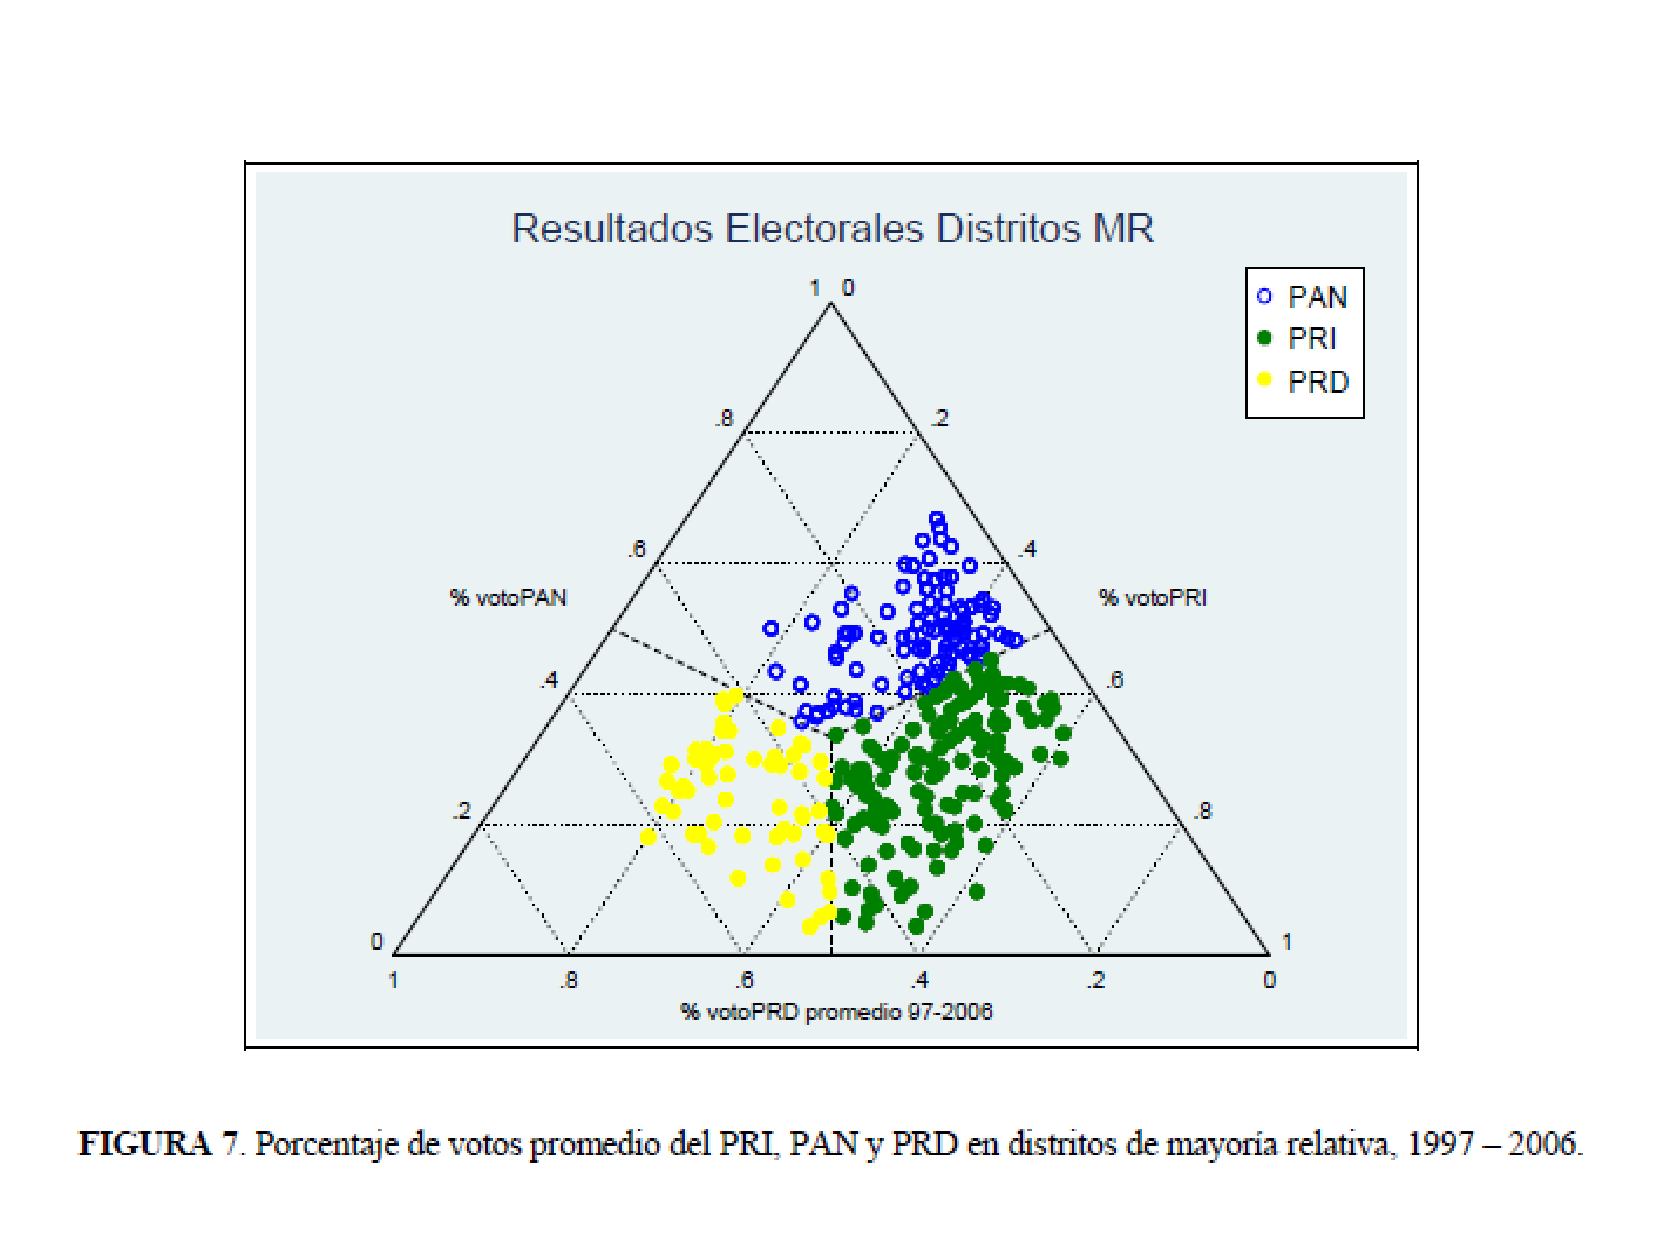
\includegraphics[width=.9\textwidth]{aparicio1.pdf} \\
\end{center}

\tiny{Source: Aparicio\&M\'arques (2010).}

}
% %%%%%%%%%%%%%%%%%%%%%%%%%%%%%%%%%%%%%%%%%%%%%%%%%%%%%%%%%%%%%%%%%%%%%%%%%%%%%%%%%%%%%%%%%%%%%%%% 
% \frame {                      % SLIDE
%     \frametitle{Party system influence}

% \begin{center}
%  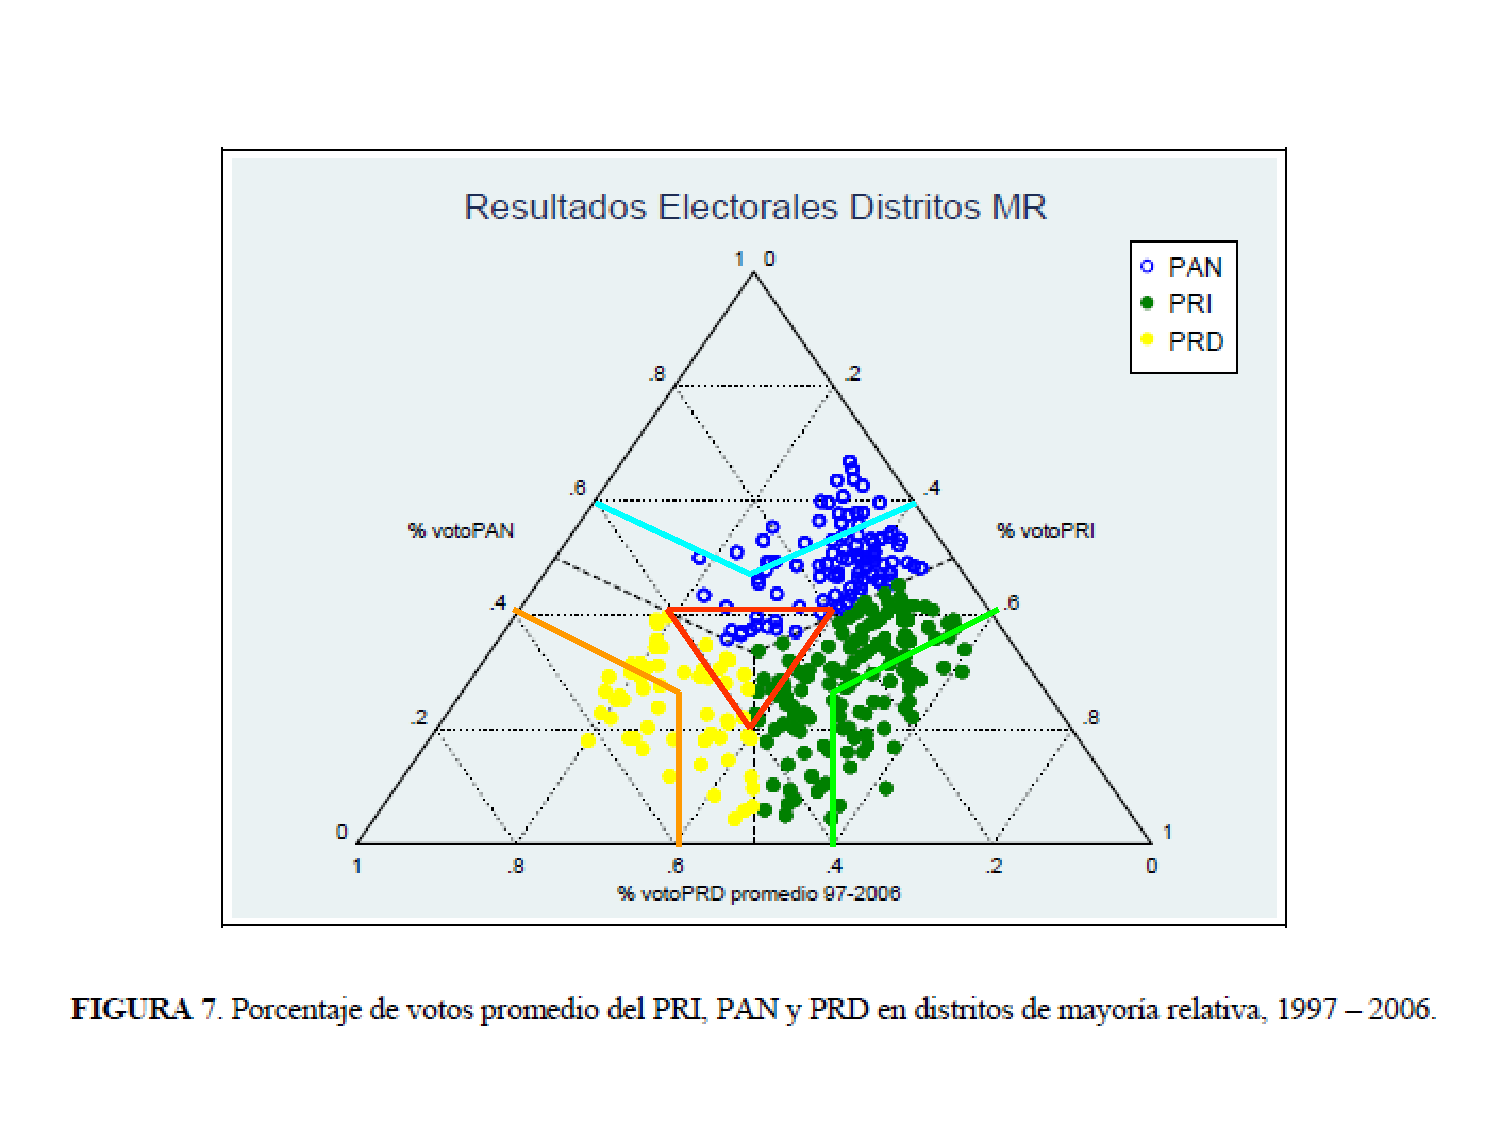
\includegraphics[width=.9\textwidth]{aparicio2.pdf} \\
% \end{center}

% \tiny{Source: Aparicio\&M\'arques (2010).}

% }
% %%%%%%%%%%%%%%%%%%%%%%%%%%%%%%%%%%%%%%%%%%%%%%%%%%%%%%%%%%%%%%%%%%%%%%%%%%%%%%%%%%%%%%%%%%%%%%%%
% \frame {                      % SLIDE
%     \frametitle{Vote trading}

% \begin{enumerate}
%     \item Efficient secret of Woldenberg council. Ugalde-Vald\'es
%     councils?
%     \item Differences in voting patterns \\
%     1996--1998 high unanimity, high divisiveness \\
%     1998--2003 low unanimity, low divisiveness \\
%     2003--2010 high unanimity, high divisiveness
% \end{enumerate}

% }
% %%%%%%%%%%%%%%%%%%%%%%%%%%%%%%%%%%%%%%%%%%%%%%%%%%%%%%%%%%%%%%%%%%%%%%%%%%%%%%%%%%%%%%%%%%%%%%%%
% \frame {                      % SLIDE
%     \frametitle{Vote winsize (incl.\ unanimous votes)}

% \begin{center}
%  \includegraphics[width=\textwidth]{c:/data/rollcall/ife_cg/graphs/winsizeStackUnan.pdf} \\
% \end{center}

% }
% %%%%%%%%%%%%%%%%%%%%%%%%%%%%%%%%%%%%%%%%%%%%%%%%%%%%%%%%%%%%%%%%%%%%%%%%%%%%%%%%%%%%%%%%%%%%%%%%
% \frame {                      % SLIDE
%     \frametitle{Vote winsize (contested votes only)}

% \begin{center}
%  \includegraphics[width=\textwidth]{c:/data/rollcall/ife_cg/graphs/winsizeStackCont.pdf} \\
% \end{center}

% }

% %%%%%%%%%%%%%%%%%%%%%%%%%%%%%%%%%%%%%%%%%%%%%%%%%%%%%%%%%%%%%%%%%%%%%%%%%%%%%%%%%%%%%%%%%%%%%%%%
% \frame {                      % SLIDE
%     \frametitle{Committee system}

% \begin{enumerate}
%     \item No majority on council
%     \item Divergent party sponsors
%     \item Self-selection to committees --- permanent allocation
%     (with barganing)
%     \item Closed rule (few modifications)
%     \item Rules change in 2007: forced rotation
%     \item 1996--2007 Different configurations on committees (strong
%     v.\ weak chairs)
%     \item Patrols v.\ alarms
%     \item test for indiv.\ committees, chairs, committee
%     configuration, party signals, TRIFE interference
% \end{enumerate}

% }
%%%%%%%%%%%%%%%%%%%%%%%%%%%%%%%%%%%%%%%%%%%%%%%%%%%%%%%%%%%%%%%%%%%%%%%%%%%%%%%%%%%%%%%%%%%%%%%%

\frame {                      % SLIDE

    \frametitle{Wrap up}

\begin{enumerate}

\item Preliminary inspection shows some promising routes

\item Ideal points in IFE move considerably. Short-term shocks and
long-term drift

\item Movement seems tied to representation
considerations \\ (change in principal; less agenda power)

\item Next: kernel smoother; committee-plenary interactions

\end{enumerate}

\pause

\center{\textbf{Thank you!}}

}
%%%%%%%%%%%%%%%%%%%%%%%%%%%%%%%%%%%%%%%%%%%%%%%%%%%%%%%%%%%%%%%%%%%%%%%%%%%%%%%%%%%%%%%%%%%%%%%%
\end{document}
%%%%%%%%%%%%%%%%%%%%%%%%%%%%%%%%%%%%%%%%%%%%%%%%%%%%%%%%%%%%%%%%%%%%%%%%%%%%%%%%%%%%%%%%%%%%%%%%


\frame {                      % SLIDE

    \frametitle{Answer 1: IFE}

 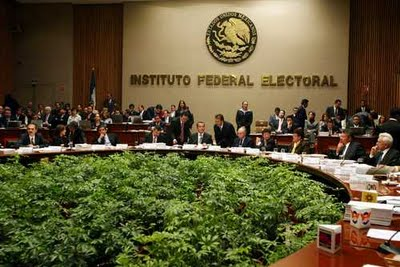
\includegraphics[width=\textwidth]{ifeCG.jpg}

}

%%%%%%%%%%%%%%%%%%%%%%%%%%%%%%%%%%%%%%%%%%%%%%%%%%%%%%%%%%%%%%%%%%%%%%%%%%%%%%%%%%%%%%%%%%%%%%%%
\frame {                      % SLIDE

    \frametitle{IFE's success story: conventional arguments}

\begin{itemize}

\item<1-> IFE as \emph{ombusdman} (Eisenstadt, Ackerman).

\item<1-> Autonomy from executive power.

\item<1-> Budget and mandate security.

\item<1-> Partisan appointment of councilors, but without inevitable bias in behavior (Schedler, Woldenberg).

\end{itemize}

\pause
\bigskip

\begin{center}
Autonomy \& impartiality $\rightarrow$ citizen trust
\end{center}

}

%%%%%%%%%%%%%%%%%%%%%%%%%%%%%%%%%%%%%%%%%%%%%%%%%%%%%%%%%%%%%%%%%%%%%%%%%%%%%%%%%%%%%%%%%%%%%%%%
\frame {                      % SLIDE

    \frametitle{Mitigating agency costs (Kiewiet \& McCubbins)}

\begin{enumerate}
    \item Formal rules to appoint councilors.
    \item Informal rules (vetoes, quotas).
    \item Party signaling in committees and Council.
    \item Appeals to election tribunal (TRIFE).
    \item Impeachment threats, election reform (nuclear option).
    \item Party capture of former councilors.
\end{enumerate}

}

%%%%%%%%%%%%%%%%%%%%%%%%%%%%%%%%%%%%%%%%%%%%%%%%%%%%%%%%%%%%%%%%%%%%%%%%%%%%%%%%%%%%%%%%%%%%%%%%
\frame {                      % SLIDE
    \frametitle{Results: contingents}

\begin{center}
 \includegraphics[width=.75\textwidth]{c:/data/rollcall/ife_cg/graphs/WoContingentes.pdf} \\
\end{center}

}
%%%%%%%%%%%%%%%%%%%%%%%%%%%%%%%%%%%%%%%%%%%%%%%%%%%%%%%%%%%%%%%%%%%%%%%%%%%%%%%%%%%%%%%%%%%%%%%%
\frame {                      % SLIDE
    \frametitle{Results: contingents}

\begin{center}
 \includegraphics[width=.75\textwidth]{c:/data/rollcall/ife_cg/graphs/UgValContingentes.pdf} \\
\end{center}

}
%%%%%%%%%%%%%%%%%%%%%%%%%%%%%%%%%%%%%%%%%%%%%%%%%%%%%%%%%%%%%%%%%%%%%%%%%%%%%%%%%%%%%%%%%%%%%%%%
\frame {                      % SLIDE
    \frametitle{Determinants of drift}

Why do ideal points move?

\bigskip

If voting were sincere $\rightarrow$ ideology drift.

\bigskip

But strategic factors abound.

}
%%%%%%%%%%%%%%%%%%%%%%%%%%%%%%%%%%%%%%%%%%%%%%%%%%%%%%%%%%%%%%%%%%%%%%%%%%%%%%%%%%%%%%%%%%%%%%%%
\frame {                      % SLIDE
    \frametitle{Results: clustering}

\begin{center}
 \includegraphics[width=.75\textwidth]{c:/data/rollcall/ife_cg/graphs/ugvalStackPRD.pdf} \\
\end{center}

}
%%%%%%%%%%%%%%%%%%%%%%%%%%%%%%%%%%%%%%%%%%%%%%%%%%%%%%%%%%%%%%%%%%%%%%%%%%%%%%%%%%%%%%%%%%%%%%%%
\frame {                      % SLIDE
    \frametitle{Vote winsize (including unanimous votes)}

\begin{center}
 \includegraphics[width=\textwidth]{c:/data/rollcall/ife_cg/graphs/winsizeUnan.pdf} \\
\end{center}

}
%%%%%%%%%%%%%%%%%%%%%%%%%%%%%%%%%%%%%%%%%%%%%%%%%%%%%%%%%%%%%%%%%%%%%%%%%%%%%%%%%%%%%%%%%%%%%%%%
\frame {                      % SLIDE
    \frametitle{Vote winsize (contested votes only)}

\begin{center}
 \includegraphics[width=\textwidth]{c:/data/rollcall/ife_cg/graphs/winsizeCont.pdf} \\
\end{center}

}
%%%%%%%%%%%%%%%%%%%%%%%%%%%%%%%%%%%%%%%%%%%%%%%%%%%%%%%%%%%%%%%%%%%%%%%%%%%%%%%%%%%%%%%%%%%%%%%%
\end{document}
%%%%%%%%%%%%%%%%%%%%%%%%%%%%%%%%%%%%%%%%%%%%%%%%%%%%%%%%%%%%%%%%%%%%%%%%%%%%%%%%%%%%%%%%%%%%%%%%
\frame {                      % SLIDE

    \frametitle{Dynamic ideal point estimation}

\begin{itemize}

\item<1-> US Supreme Court Justices need to please no one to keep their
job (Federalist 73).

\item<2-> Free to change opinion, esp.\ over long haul.

\item<3-> Evidence that they do, a lot (Martin\&Quinn).

\item<4-> Members of representative bodies don't enjoy that liberty. \\
Do their ideal points move over time? If so, why?

\end{itemize}

\pause \pause \pause \pause
\bigskip

\begin{block}{Areas we explore}
    \begin{enumerate}
        \item<5-> What is recovered by ideal point estimation?
        (Poole\&Rosenthal, Snyder et al.)
        \item<6-> What is behind ideal point drift? (McNollgast etc.)
        \item<7-> How to model/estimate
        \textbf{in}sincere voting? (Spirling\&McLean)
    \end{enumerate}
\end{block}

}

%%%%%%%%%%%%%%%%%%%%%%%%%%%%%%%%%%%%%%%%%%%%%%%%%%%%%%%%%%%%%%%%%%%%%%%%%%%%%%%%%%%%%%%%%%%%%%%%

\frame {                      % SLIDE

    \frametitle{Dynamic ideal point estimates}

 \begin{center}
  \begin{tabular}{cc}
    \includegraphics[width=.5\textwidth]{w.pdf} &
    \includegraphics[width=.5\textwidth]{u.pdf} \\
  \end{tabular}
  \footnotesize{\textcolor{white}{Colors distinguish sponsoring party, triangles expected Council median.}}
 \end{center}

}

%%%%%%%%%%%%%%%%%%%%%%%%%%%%%%%%%%%%%%%%%%%%%%%%%%%%%%%%%%%%%%%%%%%%%%%%%%%%%%%%%%%%%%%%%%%%%%%%

\frame {                      % SLIDE

    \frametitle{Dynamic ideal point estimates}

 \begin{center}
  \begin{tabular}{cc}
    \includegraphics[width=.5\textwidth]{wCol.pdf} &
    \includegraphics[width=.5\textwidth]{uCol.pdf} \\
  \end{tabular}
  \footnotesize{\textcolor{blue}{PAN}, \textcolor{red}{PRI}, \textcolor{yellow}{PRD}.}
 \end{center}

}

%%%%%%%%%%%%%%%%%%%%%%%%%%%%%%%%%%%%%%%%%%%%%%%%%%%%%%%%%%%%%%%%%%%%%%%%%%%%%%%%%%%%%%%%%%%%%%%%

\frame {                      % SLIDE

    \frametitle{Dynamic ideal point estimates}

 \begin{center}
  \begin{tabular}{cc}
    \includegraphics[width=.5\textwidth]{wColNam.pdf} &
    \includegraphics[width=.5\textwidth]{uColNam.pdf} \\
  \end{tabular}
  \footnotesize{\textcolor{blue}{PAN}, \textcolor{red}{PRI}, \textcolor{yellow}{PRD}.}
 \end{center}

}

%%%%%%%%%%%%%%%%%%%%%%%%%%%%%%%%%%%%%%%%%%%%%%%%%%%%%%%%%%%%%%%%%%%%%%%%%%%%%%%%%%%%%%%%%%%%%%%%

\frame {                      % SLIDE

    \frametitle{Drift patterns}

 \begin{center}
  \begin{tabular}{cc}
    \includegraphics[width=.5\textwidth]{c:/data/rollcall/ife_cg/graphs/driftW.pdf}
    &
    \includegraphics[width=.5\textwidth]{c:/data/rollcall/ife_cg/graphs/driftU.pdf} \\
  \end{tabular}
 \footnotesize{Grey bands = mean absolute drift $\pm$ 1 std.\ dev.}
 \end{center}

}


%%%%%%%%%%%%%%%%%%%%%%%%%%%%%%%%%%%%%%%%%%%%%%%%%%%%%%%%%%%%%%%%%%%%%%%%%%%%%%%%%%%%%%%%%%%%%%%%

\frame {                      % SLIDE

    \frametitle{Food for thought}

\begin{enumerate}

\item<1-> Ideal points in IFE move as much as in Supreme Court.

\item<2-> Movement seems tied to strategic
considerations \\ (change in principal; less agenda power).

\item<3-> Insincere voting is a problem to infer ideology. \\
Not a problem if ideal points taken literally (voting record).

\item<4-> Plan is to model/estimate strategic considerations.

\item<5-> Peress 2009 on small chamber estimators.

\end{enumerate}

\pause \pause \pause \pause \pause

\center{\textbf{Thank you!}}

}

%%%%%%%%%%%%%%%%%%%%%%%%%%%%%%%%%%%%%%%%%%%%%%%%%%%%%%%%%%%%%%%%%%%%%%%%%%%%%%%%%%%%%%%%%%%%%%%%

\frame {                      % SLIDE

    \frametitle{Case study: Mexico's Federal Election Institute}

 \begin{center}
    \includegraphics[width=\textwidth]{c:/data/rollcall/ife_cg/graphs/all+divVotsSemestre.pdf} \\
 \end{center}

}

%%%%%%%%%%%%%%%%%%%%%%%%%%%%%%%%%%%%%%%%%%%%%%%%%%%%%%%%%%%%%%%%%%%%%%%%%%%%%%%%%%%%%%%%%%%%%%%%

\frame {                      % SLIDE

    \frametitle{$x_{j,t}$ estimates with .80 credible ranges}

 \begin{center}
  \begin{tabular}{cc}
    \textbf{Periods I and II} &  \textbf{Period III} \\
    \includegraphics[width=.48\textwidth]{c:/data/rollcall/ife_cg/graphs/1dimDynWold9703jmayorPrecision.pdf}
    &
    \includegraphics[width=.48\textwidth]{c:/data/rollcall/ife_cg/graphs/1dimDynUgalde0307jmayorPrecision.pdf}
    \\
  \end{tabular}
 \end{center}

}

\end{document}
